\begin{appendices}

\chapter{Matrix Representation of MOC}
\label{app:matrix-moc}

This appendix focuses on how to solve the \ac{MOC} system of equations, focusing on the flat source approximation, as the equations are far simpler. However, a linear source approximation would lead to a similar discussion. In Chapter~\ref{chap:moc}, Eq.~\ref{eqn:angular-flux-var} and Eq.~\ref{eqn:average-flux} provided ways to calculate the angular fluxes and scalar fluxes, respectively. The source can be computed from the scalar fluxes with Eq.~\ref{eqn:source-discr}. This forms a system of equations that can be solved to determine the neutron distribution inside a nuclear reactor core. 

In this discussion, the problem will be cast as a set of matrix equations that could theoretically be solved with common linear algebra packages. However, this discussion will show that blindly solving the system of equations with a general linear algebra package is computationally infeasible since it loses sight of inherent structure the physics-based approach naturally captures.

The system of equations to be solved is formed by Eq.~\ref{eqn:source-discr}, Eq.~\ref{eqn:angular-flux-var}, and Eq.~\ref{eqn:average-flux}. Turning Eq.~\ref{eqn:source-discr} into matrix form, a fission matrix $F$ and a scattering matrix $S$ are defined such that
\begin{equation}
\mathbf{q} = \frac{1}{k} F \boldsymbol{\phi} + S \boldsymbol{\phi}
\label{eqn:matrix-source-calc}
\end{equation}
where $\mathbf{q}$ is a vector of size $M$ containing all neutron sources and $\boldsymbol{\phi}$ is a vector of size $M$ containing all scalar fluxes. Since there must be a neutron source and scalar flux for every source region and every energy group, $M = L G$ where $L$ is the number of source regions and $G$ is the number of groups. The scalar fluxes $\boldsymbol{\phi}$ as well as the sources $\mathbf{q}$ are ordered such that they are contiguous in group with the index calculated as $i G + g$. In the context of this discussion, elements relating to region quantities are indexed by source region $i$ and group $g$, yielding the following definitions for the fission matrix $F$ and scattering matrix $S$ as
\begin{eqnarray}
F_{\left(i, g\right), \, \left(i, g'\right)} = \frac{1}{4\pi} \chi_{i,g} \nu \Sigma_f^{i,g'}
\label{eqn:fission-matrix}
\end{eqnarray}
and
\begin{eqnarray}
S_{\left(i, g\right), \, \left(i, g'\right)} = \frac{1}{4\pi} \Sigma_s^{i,g' \rightarrow g}
\label{eqn:scattering-matrix}
\end{eqnarray}
where all other unspecified matrix elements are zero. Both of these matrices are of size $M \times M$ and sparse since there are no inter-regional terms.

The relationship in Eq.~\ref{eqn:angular-flux-var} can be rearranged to form the relationship in Eq.~\ref{eqn:re-angular-flux-var-disc}. This form is much easier to work with in the translation to matrix definitions.
\begin{equation}
\psi^{t,\varsigma}_g(0) \left(\frac{F_1\left(\Sigma_{t}^{i,g} s \right) - 1}{F_1\left(\Sigma_{t}^{i,g} s \right)}\right) + \psi_g^{t,\varsigma}(s) \left(\frac{1}{F_1\left(\Sigma_{t}^{i,g} s \right)}\right) = \frac{q^0_{i,g}}{\Sigma_{t}^{i,g}}
\label{eqn:re-angular-flux-var-disc}
\end{equation}
This relationship can be turned into matrix form by defining an angular flux vector $\boldsymbol{\psi}$ that contains all outgoing angular fluxes. This is represented in Eq.~\ref{eqn:matrix-attn} by an angular flux transport matrix $T$ defining relationships between angular fluxes, a source selection matrix $H$ which selects the source of the region being traversed, and a diagonal matrix $U$ containing the total cross-sections which scale the source appropriately to match the relationship in Eq.~\ref{eqn:re-angular-flux-var-disc}.
\begin{equation}
T \boldsymbol{\psi} = H U^{-1} \mathbf{q}
\label{eqn:matrix-attn}
\end{equation}
The number of angular fluxes is $N = \beta L G$ where $\beta$ is the average number of track crossings per source region. Since there must be a significant number of track crossings per region for convergence we expect $N >> M$. $T$ is size $N \times N$ as it defines relationships between angular fluxes, the size of $H$ is $N \times M$ since for each angular flux pair it must pick out the appropriate source region, and the size of $U$ is $M \times M$ since it relates only to the source regions. The elements relating to angular flux quantities are indexed by track $t$, segment $\varsigma$, and group $g$. For notational convenience, a function $R$ is created which maps a track $t$ and segment number $\varsigma$ to the traversed region $R(t,\varsigma)$. The source selection matrix $H$ can therefore be defined as
\begin{equation}
H_{\left(t,\varsigma,g\right), \, \left(R(t,\varsigma), g\right)} = 1.
\label{eqn:source-selection-matrix}
\end{equation}
This matrix therefore, has only one non-zero value per row, indicating which region is being traversed, relating track-based quantities such as angular fluxes to region based quantities such as the scalar fluxes. Its transpose similarly relates the regions to the tracks traversing the region. The matrix $H^T H$ is a $M \times M$ diagonal matrix with each diagonal element representing the number of tracks that traverse the region multiplied by the number of groups. Since it is diagonal, it is easily invertible, which will be important in the later discussion.
The diagonal matrix $U$ containing the total cross-sections is defined by
\begin{equation}
U_{\left(i, g\right), \, \left(i, g\right)} = \Sigma_t^{i,g}.
\label{eqn:total-xs-matrix}
\end{equation}
The angular flux transport matrix $T$ is defined by
\begin{equation}
T_{\left(t,\varsigma,g\right), \, \left(t, \varsigma, g\right)} = \frac{1}{F_1\left(\Sigma_{t}^{R(t,\varsigma),g} \ell_{t,\varsigma}\right)}
\label{eqn:angular-flux-transport-matrix-1}
\end{equation}
and
\begin{equation}
T_{\left(t,\varsigma,g\right), \, \left(t, \varsigma-1, g\right)} = \frac{F_1\left(\Sigma_{t}^{R(t,\varsigma),g} \ell_{t,\varsigma}\right) - 1}{F_1\left(\Sigma_{t}^{R(t,\varsigma),g} \ell_{t,\varsigma}\right)}.
\label{eqn:angular-flux-transport-matrix-2}
\end{equation}
Again, all non-specified quantities are zero.

Lastly, Eq.~\ref{eqn:average-flux} describes how the scalar flux is calculated in terms of both a weighted sum of angular fluxes and the neutron source. Specifically, an angular flux weighting matrix $W$ of size $M \times N$ is defined such that
\begin{equation}
\boldsymbol{\phi} = U^{-1}\mathbf{q} + U^{-1} W \boldsymbol{\psi}.
\label{eqn:matrix-flux-calc}
\end{equation}
In order to expose its structure, $W$ is expressed as a multiplication of matrices
\begin{equation}
W = V^{-1} H^T \tilde{W}
\end{equation}
where the volume matrix $V$ is a $M \times M$ diagonal matrix containing region volumes as
\begin{equation}
V_{\left(i, g\right), \, \left(i, g\right)} = V_i
\end{equation}
and $\tilde{W}$ is an $N \times N$ matrix defined by
\begin{equation}
\tilde{W}_{\left(t,\varsigma,g\right), \, \left(t, \varsigma, g\right)} = -w_{t}
\end{equation}
and
\begin{equation}
\tilde{W}_{\left(t,\varsigma,g\right), \, \left(t, \varsigma-1, g\right)} = w_{t}
\end{equation}
with all other elements being zero. Now that all matrix elements have been defined, the transport equation can be written as a matrix eigenvalue problem. Combining Eq.~\ref{eqn:matrix-source-calc} and Eq.~\ref{eqn:matrix-flux-calc} yields
\begin{equation}
\boldsymbol{\phi} = U^{-1} \left(\frac{1}{k} F + S \right) \boldsymbol{\phi} + U^{-1} W \boldsymbol{\psi}
\end{equation}
which combined with Eq.~\ref{eqn:matrix-attn} yields
\begin{equation}
\boldsymbol{\phi} = U^{-1}\left( I + W T^{-1} H U^{-1}\right) \left(\frac{1}{k} F + S \right) \boldsymbol{\phi}
\label{eqn:moc-matrix-form}
\end{equation}
where $I$ is the identity matrix of dimension $M \times M$. This relationship can be further simplified by defining a matrix $J$ such that
\begin{equation}
J = U^{-1}\left( I + W T^{-1} H U^{-1}\right)
\end{equation}
leading to the expression
\begin{equation}
\boldsymbol{\phi} = J \left(\frac{1}{k} F + S \right) \boldsymbol{\phi}
\label{eq:app-transport-simplified}
\end{equation}
This results in the generalized eigenvalue equation given in Eq.~\ref{eqn:gen-eig}
\begin{equation}
A \boldsymbol{\phi} = k B \boldsymbol{\phi}
\label{eqn:gen-eig}
\end{equation}
where
\begin{equation}
A = JF
\end{equation}
and
\begin{equation}
B = I - JS.
\end{equation}
This can of course be turned into a regular eigenvalue problem by explicitly taking the inverse as
\begin{equation}
B^{-1}A \boldsymbol{\phi} = k \boldsymbol{\phi}.
\label{eqn:eig}
\end{equation}
At this point, the matrix $B^{-1}A$ could be explicitly calculated and then input into any standard eigenvalue solver. However, taking matrix inverses is very computationally intense, especially due to the internal structure of $A$ and $B$. Specifically, since $J$ involves the inverse of $T$, even the explicit computation of its elements is infeasible. Therefore, doing this would be very unwise. Even if a generalized eigenvalue solver is available capable of solving equations of the form given in Eq.~\ref{eqn:gen-eig}, the problem would still rely on computing explicit components of $J$. Even though the steady-state neutron transport equation is an eigenvalue problem defined in terms of the angular fluxes, they only enter the equation implicitly with the inversion of $T$. 

%Moreover, the reaction rates of interest are defined in terms of the scalar fluxes. From angular fluxes, it is simple to calculate the scalar fluxes. This structure is an indication that explicitly solving for the full vector of angular fluxes is unnecessary.

Therefore, instead of using a common eigenvalue solution technique, a variation of fixed point iteration termed \textit{source iteration} is chosen to solve the system. In this procedure, the relationship in Eq.~\ref{eqn:moc-matrix-form} is used with the right hand side of the equation lagged as
\begin{equation}
\boldsymbol{\phi}_{n+1} = U^{-1}\left( I + W T^{-1} H U^{-1}\right) \left(\frac{1}{k_n} F + S \right) \boldsymbol{\phi}_n
\end{equation}
where the subscript $n$ indicates iteration number. Mechanically, the process iterates over estimations of the neutron source, calculating the corresponding fluxes. First, an initial flux distribution is guessed along with a value for the eigenvalue $k$. At the start of each iteration, the source distribution $\mathbf{q}$ is calculated using Eq.~\ref{eqn:matrix-source-calc} from the current guess of scalar fluxes $\boldsymbol{\phi}$ and eigenvalue $k$. Then, during the \textit{transport sweep}, new angular fluxes are computed as
\begin{equation}
\boldsymbol{\psi} = T^{-1} H U^{-1} \mathbf{q}.
\end{equation}
First, the computation of $HU^{-1}\mathbf{q}$ is trivial since $H$ is just the source selection matrix and $U$ is diagonal. Physically, this just relates to selecting the source region being traversed and calculating the source divided by the total cross-section.

Due to the simple structure of $T$, solving its \textit{implicit} inversion is rather simple for a matrix of its size. $T$ has just one element on the diagonal and one off-diagonal element per row. However, since the size of $T$ is so large, any operation involving the matrix is still expensive. Note that the angular fluxes are only related to their associated connecting angular flux. For some boundary conditions (e.g. reflective), the connecting angular flux might be from another track. This could cause the inversion to be more difficult. If all boundaries have this characteristic, all the angular fluxes within a cycle of connecting tracks would be dependent on each other.

To alleviate this issue, the angular fluxes at boundaries are approximated by the calculated angular flux at the boundary from the previous iteration. Specifically, the relationship in Eq.~\ref{eqn:angular_flux_boundary} relating connecting angular fluxes at the start of a track is approximated by
\begin{dmath}
	\psi_g^{t,1}(0) = \widetilde{\psi}_g^{C(t),S(C(t))}(\ell_{C(t),S(C(t))})
\end{dmath}
where $\widetilde{\psi}$ represents the calculated angular fluxes from the previous iteration so that $\widetilde{\psi}_g^{C(t),S(C(t))}$ is the angular flux of the connecting track from the previous iteration. This transformation allows the inversion of $T$ to be calculated using an altered matrix $\tilde{T}$ which lacks dependency between different tracks, then adding the contribution of the previous iteration angular fluxes, if applicable. The structure of $\tilde{T}$ is block-diagonal and within each block the matrix is upper triangular. Physically this means that all tracks can be calculated independently of each other during an iteration. For each track, the angular fluxes can be solved sequentially by segment. This is where the \textit{transport sweep} owes its name as the algorithm simply sweeps over segments. Since each row has at most two elements, very little calculation is required for each angular flux. 

During this process, it is noted that only the boundary angular fluxes along with the neutron source are needed to determine all angular fluxes. Therefore, non-boundary angular fluxes are computed on-the-fly. Furthermore, the elements of $T$ are re-computed on-the-fly. Once an angular flux is computed, its contribution to the scalar fluxes is tallied before it is discarded, since the computation of the scalar fluxes $\boldsymbol{\phi}$ relies on a weighted sum of the full angular flux vector $\boldsymbol{\psi}$.

After the transport sweep, the source is added to the scalar flux tally, consistent with Eq.~\ref{eqn:matrix-flux-calc}, to produce a new estimate of the scalar fluxes $\boldsymbol{\phi}$. To form a new estimate of $k$, note that
\begin{equation}
T \boldsymbol{\psi} = \frac{1}{k} H U^{-1} F \boldsymbol{\phi} + H U^{-1} S \boldsymbol{\phi}
\end{equation}
which then is re-arranged and multiplied with a vector of ones $\mathbb{1}_M$ of length $M$ as
\begin{equation}
\mathbb{1}_M^T U H_{\text{left}}^{-1} T \boldsymbol{\psi}  = \frac{1}{k} \mathbb{1}_M^T  F \boldsymbol{\phi} + \mathbb{1}_M^T  S \boldsymbol{\phi}.
\end{equation}
Since $H$ is rectangular, it cannot be simply inverted. But since it is of full rank, $H^T H$ can be inverted. From the previous discussion of $H$, recall that $H^T H$ is diagonal so its inversion is simple. Therefore the left inverse $H_{\text{left}}^{-1}$ of matrix $H$ is defined to be
\begin{equation}
H_{\text{left}}^{-1} = \left(H^T H\right)^{-1} H^T.
\end{equation}
This allows the eigenvalue $k$ to be computed as
\begin{equation}
k = \frac{\mathbb{1}_M^T F \boldsymbol{\phi}}{\mathbb{1}_M^T  U H_{\text{left}}^{-1} T \boldsymbol{\psi} - \mathbb{1}_M^T S \boldsymbol{\phi}}.
\end{equation}
Combining Eq.~\ref{eqn:matrix-attn} and Eq.~\ref{eqn:matrix-flux-calc}, note that
\begin{equation}
U H_{\text{left}}^{-1} T \boldsymbol{\psi} = U \boldsymbol{\phi} - W \boldsymbol{\psi}
\end{equation}
and therefore
\begin{equation}
k = \frac{\mathbb{1}_M^T F \boldsymbol{\phi}}{\mathbb{1}_M^T \left(U - S \right) \boldsymbol{\phi} - \mathbb{1}_M^T W \boldsymbol{\psi}}.
\end{equation}
where $\mathbb{1}_M^T F \boldsymbol{\phi}$ refers to the fission rate, $\mathbb{1}_M^T \left(U - S \right) \boldsymbol{\phi}$ refers to the absorption rate, and $-\mathbb{1}_M^T W \boldsymbol{\psi}$ refers to the leakage rate. Physically, this shows that $k$ is simply a ratio of neutron production to neutron loss terms.

Notice that each source iteration relies on simply taking the inverse of the transport matrix $T$ rather than the full $B$ matrix, which includes the scattering matrix, as would normally be taken during an eigenvalue solver, e.g. power iteration. While this choice does ease the computational burden of each iteration, it also requires many more iterations to converge to the correct solution as each iteration does little work in resolving the angular fluxes as the scattering matrix is not included in the inversion. 

Physically, this relates to not treating the scattering source as directly coupled to the total neutron source. Therefore, un-accelerated \ac{MOC} is inherently plagued by slow convergence. In OpenMOC, \ac{CMFD} acceleration is used to resolve the issue of slow convergence for source iteration, as described in Appendix~\ref{app:cmfd-acceleration}. This allows for the computational burden of each iteration to be eased without giving up anything in terms of convergence rate by iteration.

\chapter{CMFD Acceleration}
\label{app:cmfd-acceleration}

Often \ac{CMFD} acceleration is necessary to achieve reasonable convergence on practical reactor physics problems~\cite{smith1983cmfd}. This appendix explains \ac{CMFD} acceleration, as implemented in OpenMOC. During \ac{CMFD} acceleration, a coarse mesh problem is solved that is consistent with the fine mesh \ac{MOC} problem. Since the coarse mesh problem can be solved quickly, it can be fully converged and used to update the \ac{MOC} solution allowing global behavior to be communicated in fewer iterations. This appendix discuss \ac{CMFD} as a multigrid method, shows how the \ac{CMFD} equations are derived from the fundamental multi-group transport equation, and then the process of applying \ac{CMFD} acceleration is discussed.

%%%%%%%%%%%%%%%%%%%%%%%%%%%%%%%%%%%%%%%%%%%%%%%%%%%%%%%%%%%%%%%%%%%%%%%%%%%%%%%
\section{Multigrid Methods}
\label{sec:multigrid}

Multigrid methods are popular in numerical analysis for solving differential equations. The fundamental idea is that global information can be transferred much quicker over a coarse mesh than a fine mesh. Using this principle multigrid methods alternate between solving the set of equations on a coarse mesh, where the problem size is reduced and information propagates much quicker, and a fine mesh where the discretization accurately captures the solution of the problem. It is vital that the coarse mesh solution be consistent with the fine mesh solution. In this context, consistency means that at convergence the coarse mesh and fine mesh solutions agree over the coarse mesh.

Multigrid methods can be structured in many different ways but they generally involve two important stages: restriction and prolongation.
\begin{itemize}
	\item \textbf{Restriction - } Collapsing the fine mesh solution down to a consistent form on a coarse mesh.
	\item \textbf{Prolongation - } Using the coarse mesh solution to interpolate corrections to the fine mesh solution.
\end{itemize}

Multigrid methods in general can involve many layers of mesh. At each layer, restriction and prolongation are used to transfer to coarser and finer mesh layers, respectively. However, for the \ac{CMFD} acceleration scheme implemented in this thesis, only two layers of mesh are used: the fine \ac{MOC} mesh and the coarse \ac{CMFD} mesh. Figure~\ref{fig:multigrid-cmfd} illustrates the process of solving the \ac{MOC} equations using \ac{CMFD} acceleration.
\begin{figure}[h!] 
	\centering 
	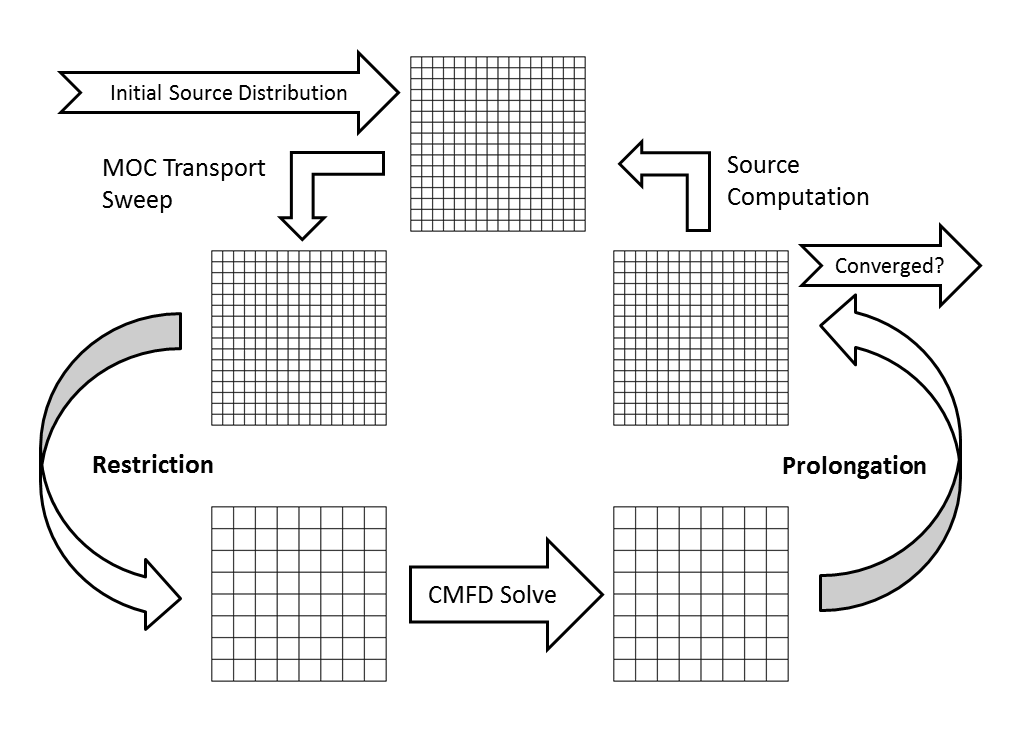
\includegraphics[width=\linewidth]{figures/multigrid-cmfd.PNG}
	\caption[]{A depiction of the multigrid approach to solving the \ac{MOC} transport equations with \ac{CMFD} acceleration.}
	\label{fig:multigrid-cmfd}
\end{figure}

One important difference between usual multigrid approaches and \ac{CMFD} is that the \ac{CMFD} equations are solved using consistent but fundamentally different equations. Instead of solving the coarse mesh problem using the same \ac{MOC} form of the neutron transport equation, where the angular space is discretized using tracks, the \ac{CMFD} equations rely on a diffusion-like formulation. This alternate form of the transport equation relies strictly on cell averaged quantities rather than having a dependence on angular directions.

%%%%%%%%%%%%%%%%%%%%%%%%%%%%%%%%%%%%%%%%%%%%%%%%%%%%%%%%%%%%%%%%%%%%%%%%%%%%%%%
\section{Derivation of the CMFD Equations}
\label{sec:cmfd-derivation}

The \ac{CMFD} equations can be derived from multi-group transport. The general concept is to turn the transport equation, which is fundamentally based on angular fluxes into a diffusion-like problem which is fundamentally based on scalar fluxes averaged over some volume in the reactor. During this process, some approximations will be introduced. However, all of these approximations introduce no bias at convergence. Therefore they do not impact solution accuracy. First recall the multigroup approximation given in Eq.~\ref{eqn:multi-group-transport}:
\begin{equation}
\mathbf{\Omega} \cdot \nabla \psi_{g}(\mathbf{r},\mathbf{\Omega}) + \Sigma_t^{g}(\mathbf{r}) \psi_{g}(\mathbf{r},\mathbf{\Omega}) = \frac{1}{4 \pi} \left( \frac{\chi_{g}\left(\mathbf{r}\right)}{k} \sum_{g'=1}^{G} \nu_{g'}\left(\mathbf{r}\right) \Sigma_f^{g'}\left(\mathbf{r}\right) \phi_{g'}\left(\mathbf{r}\right) + \, \sum_{g'=1}^G \,  \Sigma_{s}^{g' \rightarrow g}\left(\mathbf{r}\right) \phi_{g'}(\mathbf{r}) \right)
\end{equation}
To transform this equation into one based on the scalar fluxes $\phi_{g}(\mathbf{r})$ rather than the angular fluxes $\psi_{g}(\mathbf{r},\mathbf{\Omega})$, the equation is integrated over the entire $4\pi$ angular space. In doing so, recall from Eq.~\ref{eqn:scalar-flux} that the integral of angular flux over the entire angular space is simply the scalar flux, leading to the relationship in Eq.~\ref{eqn:angle_int_transport}.
\begin{equation}
\int\displaylimits_{4 \pi} d\mathbf{\Omega} \,\mathbf{\Omega} \cdot \nabla \psi_{g}(\mathbf{r},\mathbf{\Omega}) + \Sigma_t^{g}\left(\mathbf{r}\right) \phi_{g}(\mathbf{r}) = \frac{\chi_{g}\left(\mathbf{r}\right)}{k} \sum_{g'=1}^{G} \nu_{g'}\left(\mathbf{r}\right) \Sigma_f^{g'}\left(\mathbf{r}\right) \phi_{g'}(\mathbf{r}) + \, \sum_{g'=1}^G \,  \Sigma_{s}^{g' \rightarrow g}\left(\mathbf{r}\right) \phi_{g'}(\mathbf{r})
\label{eqn:angle_int_transport}
\end{equation}
Notice that only the streaming term has any dependence on the angular flux $\psi_{g}(\mathbf{r},\mathbf{\Omega})$. Since the angular variable $\mathbf{\Omega}$ is independent of the spatial variable $\mathbf{r}$, the gradient can be brought outside the integral in the streaming term as shown in Eq.~\ref{eqn:angle_int_transport_grad}.
\begin{equation}
\nabla \cdot \int\displaylimits_{4 \pi} d\mathbf{\Omega} \,\mathbf{\Omega} \psi_{g}(\mathbf{r},\mathbf{\Omega}) + \Sigma_t^{g}\left(\mathbf{r}\right) \phi_{g}(\mathbf{r}) = \frac{\chi_{g}\left(\mathbf{r}\right)}{k} \sum_{g'=1}^{G} \nu_{g'}\left(\mathbf{r}\right) \Sigma_f^{g'}\left(\mathbf{r}\right) \phi_{g'}(\mathbf{r}) + \, \sum_{g'=1}^G \,  \Sigma_{s}^{g' \rightarrow g}\left(\mathbf{r}\right) \phi_{g'}(\mathbf{r})
\label{eqn:angle_int_transport_grad}
\end{equation}
Next, the net current $J_g\left(\mathbf{r}\right)$ is defined as
\begin{equation}
J_g\left(\mathbf{r}\right) = \int\displaylimits_{4 \pi} d\mathbf{\Omega} \,\mathbf{\Omega} \psi_{g}(\mathbf{r},\mathbf{\Omega}).
\label{eqn:net_current}
\end{equation}
Inserting this definition and integrating the equation over an arbitrary volume $V$ leads to Eq.~\ref{eqn:vol_int_transport}.
\begin{equation}
\begin{split}
\int\displaylimits_{V} d\mathbf{r} \,\nabla \cdot J_g\left(\mathbf{r}\right) + \int\displaylimits_{V} d\mathbf{r} \, \Sigma_t^{g}\left(\mathbf{r}\right) \phi_{g}(\mathbf{r}) = & \\
\int\displaylimits_{V} d\mathbf{r} \, \Bigg( \frac{\chi_{g}\left(\mathbf{r}\right)}{k} \sum_{g'=1}^{G} & \nu_{g'}\left(\mathbf{r}\right) \Sigma_f^{g'}\left(\mathbf{r}\right) \phi_{g'}(\mathbf{r}) + \, \sum_{g'=1}^G \,  \Sigma_{s}^{g' \rightarrow g}\left(\mathbf{r}\right) \phi_{g'}(\mathbf{r}) \Bigg) 
\end{split}
\label{eqn:vol_int_transport}
\end{equation}
The entire geometry is then partitioned into \ac{CMFD} cells. Defining a volume $V_j$ for \ac{CMFD} cell $j$ which is the composition of a finite number of non-overlapping \ac{MOC} source regions, the transport equation can be cast in terms of the fluxes and constant cross-sections for the \ac{MOC} source regions $i$ with volumes $V_i$ as given in Eq.~\ref{eqn:cmfd_composition_moc}. 
\begin{equation}
\begin{split}
\int\displaylimits_{V_j} d\mathbf{r} \,\nabla \cdot J_g\left(\mathbf{r}\right) + & \sum_{i \in j} \int\displaylimits_{V_i} d\mathbf{r} \, \Sigma_t^{i,g} \phi_{g}(\mathbf{r}) = \\
& \sum_{i \in j} \int\displaylimits_{V_i} d\mathbf{r} \, \left( \frac{\chi_{i,g}}{k} \sum_{g'=1}^{G} \nu_{i, g'} \Sigma_f^{i,g'} \phi_{g'}(\mathbf{r}) + \sum_{g'=1}^G  \Sigma_{s}^{i, g' \rightarrow g} \phi_{g'}(\mathbf{r}) \right)
\end{split}
\label{eqn:cmfd_composition_moc}
\end{equation}
It is important to note that in this definition, \ac{CMFD} boundaries are not allowed to intersect \ac{MOC} source region boundaries. In practice, source regions with an intersecting \ac{CMFD} boundary are split so that each source region has only one \ac{CMFD} cell within its domain. Since the \ac{MOC} equations are often solved for the average flux within source regions, $\overline{\phi_{i,g}}$, the transport equation can be re-written as:
\begin{equation}
\int\displaylimits_{V_j} d\mathbf{r} \,\nabla \cdot J_g\left(\mathbf{r}\right) + \sum_{i \in j} \Sigma_t^{i,g} \overline{\phi_{i,g}} V_i = \sum_{i \in j} \left( \frac{\chi_{i,g}}{k} \sum_{g'=1}^{G} \nu_{i, g'} \Sigma_f^{i,g'} \overline{\phi_{i,g'}} V_i + \sum_{g'=1}^G   \Sigma_{s}^{i, g' \rightarrow g}\overline{\phi_{i,g'}} V_i \right)
\end{equation}
All of the variables given in this equation are present in the \ac{MOC} equations except for the net current found in the streaming term. The bounding surface of \ac{CMFD} cell $j$ is defined as $S_j$ with surface normal $\mathbf{n}$. Applying gauss-divergence theorem to the streaming term, it can be cast as a surface integral, shown in Eq.~\ref{eqn:cmfd_gauss_divergence}.
\begin{equation}
\int\displaylimits_{S \in S_j} dS \, J_g\left(\mathbf{r}\right) \cdot \mathbf{n} + \sum_{i \in j} \Sigma_t^{i,g} \overline{\phi_{i,g}} V_i = \sum_{i \in j} \left( \frac{\chi_{i,g}}{k} \sum_{g'=1}^{G} \nu_{i, g'} \Sigma_f^{i,g'} \overline{\phi_{i,g'}} V_i + \sum_{g'=1}^G   \Sigma_{s}^{i, g' \rightarrow g}\overline{\phi_{i,g'}} V_i \right)
\label{eqn:cmfd_gauss_divergence}
\end{equation}
In order to make the \ac{CMFD} problem even less computationally intense, the group structure is coarsened. A group collapse is performed in which a given \ac{CMFD} group $e$ is formed from the incorporation of one or more \ac{MOC} groups. To arrive at this relationship, the transport equation is summed over all \ac{MOC} groups $g$ within the \ac{CMFD} group $e$, shown in Eq.~\ref{eqn:cmfd_sum_groups}.
\begin{equation}
\begin{split}
\sum_{g \in e} \left( \int\displaylimits_{S \in S_j} dS \, J_g\left(\mathbf{r}\right) \cdot \mathbf{n} + \sum_{i \in j} \Sigma_t^{i,g} \overline{\phi_{i,g}} V_i \right) = & \\
\sum_{i \in j}  \Bigg( \frac{\sum_{g \in e} \chi_{i,g}}{k} \sum_{g'=1}^{G}  \nu_{i, g'} \Sigma_f^{i,g'} \overline{\phi_{i,g'}} V_i & + \sum_{g'=1}^G \left(\sum_{g \in e} \Sigma_{s}^{i, g' \rightarrow g} \right) \overline{\phi_{i,g'}} V_i \Bigg)
\end{split}
\label{eqn:cmfd_sum_groups}
\end{equation}
\ac{CMFD} cross-sections over coarse mesh and coarse group structures are defined in terms of the fine mesh \ac{MOC} quantities. The \ac{CMFD} cross-sections are given the subscript $C$ and their definitions are given in equations ~\ref{eqn:cmfd-xs-chi} -- ~\ref{eqn:cmfd-xs-total}. 
\begin{equation}
\chi_C^{j,e} = \frac{\sum_{i \in j} \left[ \left(\sum_{g \in e} \chi_{i,g} \right) \left(\sum_{g'=1}^{G} \nu_{i, g'} \Sigma_f^{i,g'} \overline{\phi_{i,g'}} V_i \right)\right]}{\sum_{i \in j} \sum_{g=1}^{G} \nu_{i, g} \Sigma_f^{i,g} \overline{\phi_{i,g}} V_i}
\label{eqn:cmfd-xs-chi}
\end{equation}
\begin{equation}
\nu_C^{j,e} \, \Sigma_{C,f}^{j,e} = \frac{\sum_{i \in j} \sum_{g \in e} \nu_{i, g} \Sigma_f^{i,g} \overline{\phi_{i,g}} V_i}{\sum_{i \in j} \sum_{g \in e} \overline{\phi_{i,g}} V_i}
\end{equation}
\begin{equation}
\Sigma_{C,s}^{j, e' \rightarrow e} = \frac{\sum_{i \in j} \sum_{g'\in e'} \left(\sum_{g \in e} \Sigma_{s}^{i, g' \rightarrow g} \right) \overline{\phi_{i,g'}} V_i}{\sum_{i \in j} \sum_{g\in e} \overline{\phi_{i,g}} V_i}
\end{equation}
\begin{equation}
\Sigma_{C,t}^{j, e} = \frac{\sum_{i \in j} \sum_{g \in e} \Sigma_{t}^{i, g} \overline{\phi_{i,g}} V_i}{\sum_{i \in j} \sum_{g\in e} \overline{\phi_{i,g}} V_i}
\label{eqn:cmfd-xs-total}
\end{equation}
Notice that these cross-sections involve a weighting over the \ac{MOC} fluxes. Therefore the \ac{CMFD} solution depends on the \ac{MOC} scalar fluxes. At convergence, there is no approximation error, allowing the \ac{CMFD} solution to be entirely consistent. \ac{CMFD} cell volumes $V_C^j$ and cell-averaged scalar fluxes $\phi_C^{j,e}$ are defined by Eq.~\ref{eqn:cmfd_volumes} and Eq.~\ref{eqn:cmfd_scalar_fluxes}, respectively.
\begin{equation}
V_C^j = \sum_{i \in j} V_i
\label{eqn:cmfd_volumes}
\end{equation}
\begin{equation}
\phi_C^{j,e} = \frac{\sum_{i \in j} \sum_{g \in e} \overline{\phi_{i,g}} V_i}{\sum_{i \in j} V_i}
\label{eqn:cmfd_scalar_fluxes}
\end{equation}
These definitions, along with the \ac{CMFD} cross-section definitions, form the basis of the restriction component of \ac{CMFD} acceleration. It is important to note that the \ac{CMFD} mesh is significantly coarser - both in space and energy -- than the \ac{MOC} mesh. A comparison of the spatial mesh is given in Figure~\ref{fig:cmfd-mesh} with the \ac{MOC} mesh on the left. The depicted mesh are the actual mesh sizes used in the final results for this thesis. The \ac{MOC} mesh is quite coarser than typical \ac{MOC} mesh due to the use of a linear source approximation. The \ac{CMFD} calculations in this thesis use pin-cell sized mesh. Even with the coarse \ac{MOC} mesh, the \ac{CMFD} mesh is significantly coarser.
\begin{figure}[h!]
	\centering
	\begin{subfigure}{0.45\textwidth}
		\centering
		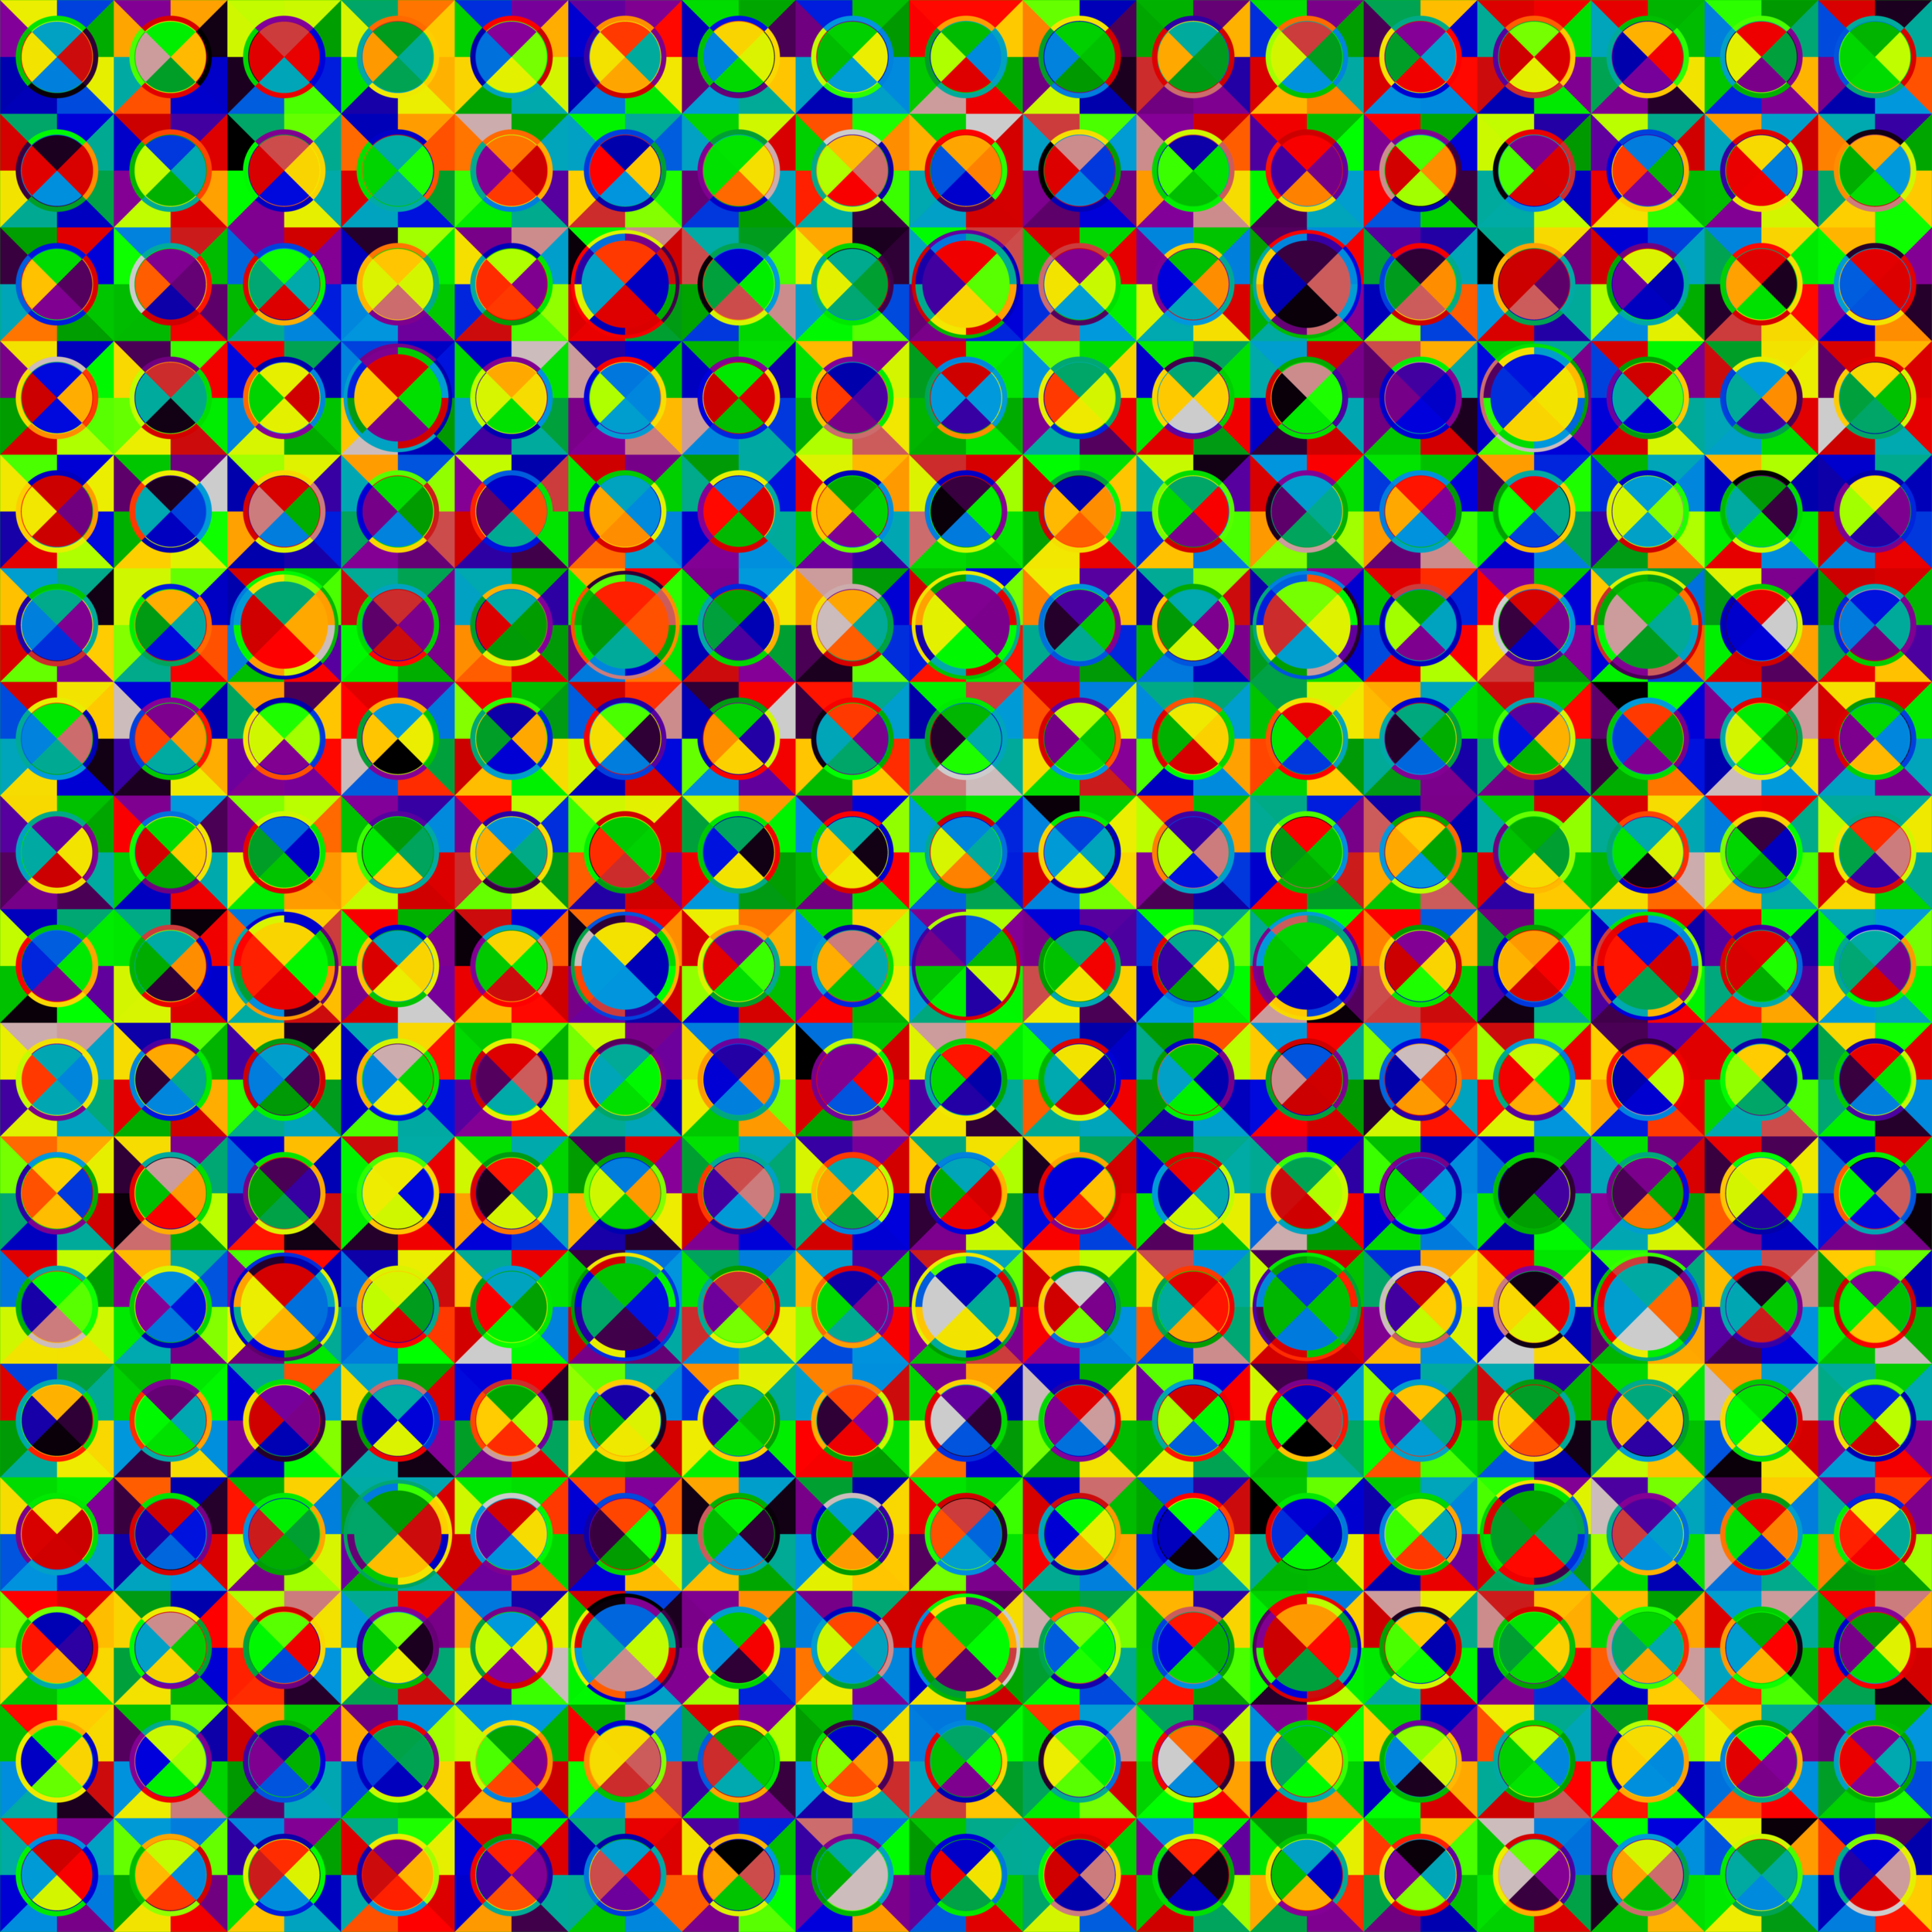
\includegraphics[width=\linewidth]{figures/old3_moc_mesh.PNG}
		\caption{}
		\label{fig:cmfd-mesh-a}
	\end{subfigure}
	\begin{subfigure}{0.45\textwidth}
		\centering
		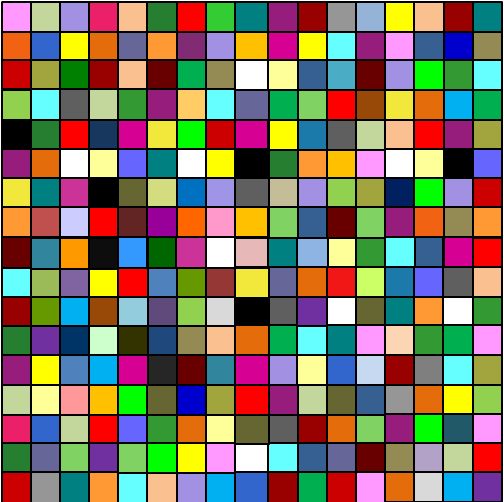
\includegraphics[width=\linewidth]{figures/cmfd_mesh.PNG}
		\caption{}
		\label{fig:cmfd-mesh-b}
	\end{subfigure}
	\caption[]{A depiction of the spatial mesh used in \ac{MOC} (a) and \ac{CMFD} (b) solvers. The mesh refinements correspond to those used in the final results for this thesis.}
	\label{fig:cmfd-mesh}
\end{figure}

For the energy condensation, the \ac{MOC} calculations in this thesis use 70 energy groups whereas the \ac{CMFD} solver uses 25 or less energy groups. The combination of coarse spatial mesh and coarse energy groups causes the \ac{CMFD} problem size to be incredibly small in comparison with the \ac{MOC} problem size. With the collapsed cross-sections on the coarse mesh, the \ac{CMFD} transport equation looks very similar to the original multi-group transport equation and is given in Eq.~\ref{eqn:cmfd_transport}.
\begin{equation}
\frac{1}{V_C^j} \sum_{g \in e} \left( \int\displaylimits_{S \in S_j} dS \, J_g\left(\mathbf{r}\right) \cdot \mathbf{n} \right) + \Sigma_{C,t}^{j,e} \phi_C^{j,e} = \frac{\chi_C^{j,e}}{k} \sum_{e'=1}^{E} \nu_C^{j, e'} \Sigma_{C,f}^{j,e'} \phi_C^{j,e'} + \sum_{e'=1}^E  \Sigma_{C,s}^{i, e' \rightarrow e} \phi_C^{j,e'}
\label{eqn:cmfd_transport}
\end{equation}
Returning to the streaming term, the entire surface $S_j$ of \ac{CMFD} cell $j$ is partitioned into $H$ surfaces that form an interface between cell $j$ and exactly one other \ac{CMFD} cell. This allows the total net current of \ac{CMFD} cell $j$ to be defined in terms of the sum over net currents over these interfacial surfaces as given in Eq.~\ref{eqn:cmfd_partial_surface_currents}.
\begin{equation}
\frac{1}{V_C^j} \sum_{g \in e} \sum_{h=1}^H \left( \int\displaylimits_{S \in S_{j,h}} dS \, J_g\left(\mathbf{r}\right) \cdot \mathbf{n} \right) + \Sigma_{C,t}^{j,e} \phi_C^{j,e} = \frac{\chi_C^{j,e}}{k} \sum_{e'=1}^{E} \nu_C^{j, e'} \Sigma_{C,f}^{j,e'} \phi_C^{j,e'} + \sum_{e'=1}^E  \Sigma_{C,s}^{i, e' \rightarrow e} \phi_C^{j,e'}
\label{eqn:cmfd_partial_surface_currents}
\end{equation}
The integrated net current over each interfacial surface for an \ac{MOC} group $g$ can be cast in terms of angular fluxes using the definition given in Eq.~\ref{eqn:net_current} to produce the relationship in Eq.~\ref{eqn:interfacial_current_def}.
\begin{equation}
\int\displaylimits_{S_{j,h}} dS \, J_g\left(\mathbf{r}\right) \cdot \mathbf{n} =  \int\displaylimits_{S \in S_{j,h}} dS \, \int\displaylimits_{4 \pi} d\mathbf{\Omega} \, \psi_{g}(\mathbf{r},\mathbf{\Omega}) \left(\mathbf{\Omega} \cdot \mathbf{n} \right)
\label{eqn:interfacial_current_def}
\end{equation}
Figure~\ref{fig:cmfd-contact-surface} shows the geometric relationship between a given \ac{MOC} track and \ac{CMFD} surfaces. This shows that the surface area penetrated on surface $S_{j,h}$ by track $t$ can be calculated as $\delta A_{t} / \left(\mathbf{\Omega} \cdot \mathbf{n}\right)$.
\begin{figure}[h!]
	\centering
	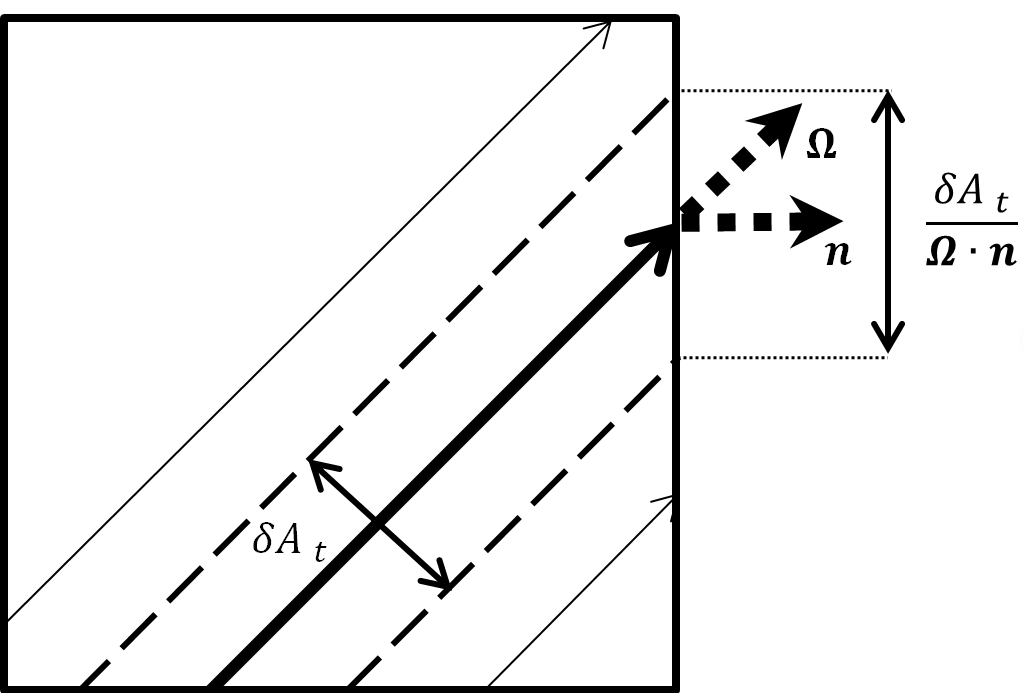
\includegraphics[width=0.5\linewidth]{figures/cmfd-contact-surface.PNG}
	\caption[]{A depiction of a \ac{CMFD} surface with normal vector $\mathbf{n}$ being penetrated by a track with cross-sectional area $\delta A_{t}$ traveling in direction $\mathbf{\Omega}$. The area of the penetrated surface area is $\delta A_{t} / \left(\mathbf{\Omega} \cdot \mathbf{n}\right)$.}
	\label{fig:cmfd-contact-surface}
\end{figure}
With this geometric relationship in mind and factoring in angular weights from Eq.~\ref{eqn:weight-def}, the integrated net current over the interfacial surface can be calculated using Eq.~\ref{eqn:moc_net_current_calc}.
%\begin{equation}
%	\int\displaylimits_{S_{j,h}} dS \, J_g\left(\mathbf{r}\right) \cdot \mathbf{n} =  \sum_{(t,s) \in S_{j,h}} \frac{w_{t}}{\mathbf{\Omega} \cdot \mathbf{n}} \psi_{g}^{t,s}(s_{j,h}) \left(\mathbf{\Omega} \cdot \mathbf{n} \right)
%\end{equation}
\begin{equation}
\int\displaylimits_{S \in S_{j,h}} dS \, J_g\left(\mathbf{r}\right) \cdot \mathbf{n} =  \sum_{(t,s) \in S_{j,h}} w_{i,t} \psi_{g}^{t,s}(s_{j,h})
\label{eqn:moc_net_current_calc}
\end{equation}
Similar to the \ac{CMFD} cross-sections, these currents are formed from the \ac{MOC} calculation, so they are only approximate until convergence. Summing over all \ac{MOC} groups $g$ within \ac{CMFD} group $e$ gives a representation for the net current $\tilde{J}_{j,h,e}$ across surface $h$ of cell $j$ for \ac{CMFD} group $e$ in Eq.~\ref{eqn:cmfd_partial_current}.
\begin{equation}
\tilde{J}_{j,h,e} = \sum_{g \in e} \sum_{(t,s) \in S_{j,h}} w_t \psi_{g}^{t,s}(s_{j,h})
\label{eqn:cmfd_partial_current}
\end{equation}
It is important to note that these estimates rely on angular fluxes. Since the entire angular flux vector is not stored explicitly, as discussed in Appendix~\ref{app:matrix-moc}, when a \ac{CMFD} surface is encountered during the \ac{MOC} transport sweep, the contribution of angular fluxes along the track to the net current on the \ac{CMFD} surface must be tallied. This is usually a relatively cheap operation, not adding much work to the transport sweep. With these calculated currents, the new transport equation is given in Eq.~\ref{eqn:transport_partial_current_1}.
\begin{equation}
\frac{1}{V_C^j} \sum_{h=1}^H \tilde{J}_{j,h,e} + \Sigma_{C,t}^{j,e} \phi_C^{j,e} = \frac{\chi_C^{j,e}}{k} \sum_{e'=1}^{E} \nu_C^{j, e'} \Sigma_{C,f}^{j,e'} \phi_C^{j,e'} + \sum_{e'=1}^E  \Sigma_{C,s}^{i, e' \rightarrow e} \phi_C^{j,e'}
\label{eqn:transport_partial_current_1}
\end{equation}
With this new representation of neutron balance, it is possible to solve for new scalar fluxes. However, this is not in the form of an eigenvalue problem since the streaming term has no dependence on the scalar flux. Therefore, new terms are introduced that relate the current to the scalar flux via diffusion coefficients. This is shown in Eq.~\ref{eqn:cmfd_current_repr}~\cite{smith1983cmfd}.
\begin{equation}
\frac{\tilde{J}_{j,h,e}}{A_{j,h}} = - u(j,h) \hat{D}_{j,e} \left(\phi_C^{I(j,h),e} - \phi_C^{j,e}\right) - \tilde{D}_{j,h,e} \left(\phi_C^{I(j,h),e} + \phi_C^{j,e}\right)
\label{eqn:cmfd_current_repr}
\end{equation}
The function $u(j,h)$ is the \textit{sense} of the surface $h$ on cell $j$, $A_{j,h}$ is the area of surface $S_{j,h}$, $\hat{D}_{j,e}$ is the surface diffusion coefficient, and $\tilde{D}_{j,h,e}$ is the nonlinear corrected diffusion coefficient. The inspiration of the first term involving $\hat{D}_{j,e}$ comes from diffusion theory. Specifically it can be calculated using Eq.~\ref{eqn:surf_diff_coef} under a \ac{CMFD} uniform mesh assumption
\begin{equation}
\hat{D}_{j,h,e} = \frac{D_{j,e} D_{I(j,h),e}}{\Delta \mathbf{r}_h \left( D_{j,e} + D_{I(j,h),e} \right)}
\label{eqn:surf_diff_coef}
\end{equation}
where $\Delta \mathbf{r}_h$ is the distance between the \ac{CMFD} cell and the interfacial surface $h$, the function $I(j,h)$ computes the index of the neighboring \ac{CMFD} cell of $j$ on surface $h$, and $D_{j,e}$ is the diffusion coefficient of cell $j$ in group $e$. Due to the uniform mesh assumption, the distance between the centroid of cell $j$ and surface $h$ is the same as that of the neighboring cell $I(j,h)$. In this thesis, the uniform mesh assumption is imposed, but a more general treatment is possible. The diffusion coefficients are defined in Eq.~\ref{eqn:cmfd_diff_coef}, with motivation from how diffusion coefficients are calculated in common nodal diffusion theory.
\begin{equation}
D_{j,e} = \frac{\sum_{i \in j} \sum_{g \in e} \frac{1}{3\Sigma_{t}^{i, g}} \overline{\phi_{i,g}} V_i}{\sum_{i \in j} \sum_{g \in e} \overline{\phi_{i,g}} V_i}
\label{eqn:cmfd_diff_coef}
\end{equation}
The sense $u(j,h)$ is calculated by Eq.~\ref{eqn:sense} where $\mathbb{1}$ is just the vector of ones in three dimensions and $\mathbf{n}_{j,h}$ is the normal vector of surface $S_{j,h}$. For a Cartesian uniform mesh, the sense is $+1$ if the surface is a positive $x$, $y$, or $z$ surface and $-1$ if it is a negative $x$, $y$, or $z$ surface.
\begin{equation}
u(j,h) = \frac{\mathbb{1} \cdot \mathbf{n}_{j,h}}{|\mathbb{1} \cdot \mathbf{n}_{j,h}|}
\label{eqn:sense}
\end{equation}
Lastly, the corrected diffusion coefficients $\tilde{D}_{j,h,e}$ are computed based on the relationship in Eq.~\ref{eqn:cmfd_current_repr} for fluxes computed after the \ac{MOC} transport sweep and before the \ac{CMFD} solve. This makes the \ac{CMFD} calculation consistent with the \ac{MOC} calculation at convergence~\cite{smith1983cmfd}. The calculation of the corrected diffusion coefficients therefore follows Eq.~\ref{eqn:cmfd_corr_dif_coef} where $\tilde{\phi}_C^{j,e}$ are the \ac{CMFD} cell-averaged scalar fluxes calculated from the \ac{MOC} iteration with the tilde indicating the quantity comes from the \ac{MOC} calculation and does not change throughout the \ac{CMFD} iterations.
\begin{equation}
\tilde{D}_{j,h,e} = \frac{-u(j, h) \hat{D}_{j,h,e} \left(\tilde{\phi}_C^{I(j,h),e} - \tilde{\phi}_C^{j,e}\right) - \frac{\tilde{J}_{j,h,e}}{A_{j,h}}}{\tilde{\phi}_C^{I(j,h),e} + \tilde{\phi}_C^{j,e}}
\label{eqn:cmfd_corr_dif_coef}
\end{equation}
Returning to balance equation and inserting the relationship for net current yields the new balance equation given in Eq.~\ref{eqn:cmfd_final_balance}.
\begin{equation}
\begin{split}
\frac{1}{V_C^j} \sum_{h=1}^H A_{j,h} \left( - u(j, h) \hat{D}_{j,e} \left(\phi_C^{I(j,h),e} - \phi_C^{j,e}\right) - \tilde{D}_{j,h,e} \left(\phi_C^{I(j,h),e} + \phi_C^{j,e}\right) \right) + \Sigma_{C,t}^{j,e} \phi_C^{j,e} = \\
\frac{\chi_C^{j,e}}{k} \sum_{e'=1}^{E} \nu_C^{j, e'} \Sigma_{C,f}^{j,e'} \phi_C^{j,e'} + \sum_{e'=1}^E  \Sigma_{C,s}^{i, e' \rightarrow e} \phi_C^{j,e'}
\end{split}
\label{eqn:cmfd_final_balance}
\end{equation}

\section{Solving the CMFD Equations for MOC Acceleration}
The \ac{CMFD} balance equation in Eq.~\ref{eqn:cmfd_final_balance} represents a physically equivalent system to solve the transport equation as the \ac{MOC} balance equation in Eq.~\ref{eqn:angular-flux-var}. Re-arranging terms in the balance equation and grouping by scalar flux yields the relationship in Eq.~\ref{eqn:cmfd_balance_grouped}.
\begin{equation}
\begin{split}
\left[\Sigma_{C,t}^{j,e} V_C^j + \sum_{h=1}^H A_{j,h} \left(u(j,h) \hat{D}_{j,e} - \tilde{D}_{j,h,e} \right) \right] \phi_C^{j,e} - \sum_{h=1}^H A_{j,h} \left( \tilde{D}_{j,h,e} + u(j,h) \hat{D}_{j,e} \right) \phi_C^{I(j,h),e} & \\ - \sum_{e'=1}^E  \Sigma_{C,s}^{i, e' \rightarrow e} V_C^j \phi_C^{j,e'} =
\frac{\chi_C^{j,e}}{k} \sum_{e'=1}^{E} \nu_C^{j, e'} \Sigma_{C,f}^{j,e'} V_C^j \phi_C^{j,e'} & \\
\end{split}
\label{eqn:cmfd_balance_grouped}
\end{equation}
This can be written in terms of a matrix eigenvalue problem by defining a scalar flux vector $\Phi_C$ which incorporates all of the \ac{CMFD} cell-averaged scalar fluxes $\phi_C^{j,e}$, a loss matrix $A$, and a multiplicative matrix $M$ in Eq.~\ref{eqn:cmfd_eigenvalue_problem}.
\begin{equation}
A \Phi_C = \frac{1}{k} M \Phi_C
\label{eqn:cmfd_eigenvalue_problem}
\end{equation}
This can be related to a regular eigenvalue problem by taking the inverse of $A$ as
\begin{equation}
A^{-1} M \Phi_C = k \Phi_C.
\end{equation}
Any common eigenvalue solver can be used to solve this system. In this thesis, simple power iteration is employed. This requires that every iteration solve a linear system. In this thesis, the linear system is solved with the red-black SOR algorithm~\cite{kords-book}. The power iteration algorithm and its application to the \ac{CMFD} equations is described later in Alg.~\ref{alg:moc-cmfd-eigenvalue-solve}.

Often, a relaxation factor is applied to the corrected diffusion coefficients in order to ensure stability~\cite{smith2002casmo}. With the relaxation factor $\omega$, the computed corrected diffusion coefficients are damped in iteration $n+1$ by
\begin{equation}
\tilde{D}_{j,h,e}^{n+1} = \omega \tilde{D}_{j,h,e}^{n+1/2} + (1-\omega) \tilde{D}_{j,h,e}^{n}
\label{eq:cmfd_damp_corr_dif_coef}
\end{equation}
where the half-iterations refer to the computed diffusion coefficient without damping, as given in Eq.~\ref{eqn:cmfd_corr_dif_coef}. The relaxation factor $\omega$ can be any real number in the interval [0,1] chosen by the user. A lower relaxation factor leads to greater stability, but also leads to slower convergence.

\section{Convergence Criteria}

Convergence for source iteration is determined when \texttt{esp-MOC} defined in Eq.~\ref{eq:eps-MOC} is reduced to $10^{-4}$ and the change in eigenvalue estimate from the previous iteration is less than 1 pcm. The same criteria is imposed for convergence with \ac{CMFD} accelerationn.

When \ac{CMFD} acceleration is applied, there are also tolerances for the \ac{CMFD} solver. Since the \ac{CMFD} equations are solved with power iteration and during each iteration a linear system is solved with red-black SOR, two \ac{CMFD} tolerances are required: the tolerance for power iteration and the tolerance for the linear solver.

If a constant tolerance were set, significant computational time could be wasted when the system is far from convergence. In the context of \ac{CMFD} acceleration for \ac{MOC}, early \ac{MOC} source iterations will have significant error in neutron sources. Therefore, the resulting \ac{CMFD} solution will also have significant error, even with strict convergence criteria. For this reason, the convergence criteria is always relative to either the current residual of the \ac{MOC} solution or the reduction in error from the starting guess. In every iteration, the starting guess is the previously converged solution, and therefore also implicitly tied to the \ac{MOC} residual.

In this thesis, the tolerance on \ac{CMFD} power iteration is chosen to be an error reduction by a factor of 0.03 from the first iteration residual. For the linear solve, an error reduction by a factor of 0.1 is required \textit{or} a neutron production residual of less than 0.01 \texttt{eps-MOC}. For both the power iteration and linear solve, a minimum of 25 iterations is enforced.

\section{Prolongation}

Once the \ac{CMFD} equations are solved, the solution is used to update \ac{MOC} fluxes, hence producing a new source for the next iteration. The updating of \ac{MOC} fluxes is the prolongation step of the \ac{CMFD} process. There are a variety of ways for which the \ac{CMFD} fluxes can be updated. One simple approach is just updating all \ac{MOC} fluxes in source region $i$ and \ac{MOC} group $g$ encompassed by \ac{CMFD} cell $j$ and \ac{CMFD} group $e$ by applying Eq.~\ref{eqn:cmfd_simple_prolongation}:
\begin{equation}
\phi_{i,g}^{\text{new}} = \phi_{i,g}^{\text{old}} \, \frac{\phi_{C, \, \text{new}}^{j,e}}{\phi_{C, \, \text{old}}^{j,e}}
\label{eqn:cmfd_simple_prolongation}
\end{equation}
where $\phi_{i,g}^{\text{new}}$ refers to the updated \ac{MOC} flux after prolongation, $\phi_{i,g}^{\text{old}}$ refers to the \ac{MOC} flux before prolongation, $\phi_{C, \, \text{old}}^{j,e'}$ refers to the \ac{CMFD} cell-averaged flux at the start of the \ac{CMFD} solution (calculated directly from the \ac{MOC} fluxes), and $\phi_{C, \, \text{new}}^{j,e'}$ refers to the \ac{CMFD} cell-averaged flux at convergence of the \ac{CMFD} solution. It is important to ensure that both new and old scalar fluxes are normalized in the same manner.

While this prolongation approach works well when the \ac{CMFD} mesh is fine, the \ac{CMFD} acceleration could be aided by interpolating the \ac{CMFD} solution if the shape is known. For the axial direction, we expect smoothly varying flux shapes due to the simplistic geometric axial structure. Therefore, the flux shape in each cell is approximated as being quadratic. Both the before and after \ac{CMFD} flux shapes are fit with a quadratic interpolation using neighboring domains. Specifically, the axial flux distribution a \ac{CMFD} cell $j$ for energy group $e$ is represented as
\begin{equation}
\begin{split}
\phi_C^{j,e}(z) \approx & \phi_C^{j-1,e}\left(\frac{\left(z-z^C_j \right)^2}{2} - \left(z-z^C_j \right) - \frac{1}{24} \right) + \phi_C^{j,e}\left(-\left(z-z^C_j \right)^2 + \frac{26}{24} \right) + \\ & \phi_C^{j+1,e}\left(\frac{\left(z-z^C_j \right)^2}{2} - \left(z-z^C_j \right) - \frac{1}{24} \right)
\end{split}
\end{equation}
for axial height $z$ with the centroid of the \ac{CMFD} cell at height $z^C_{j}$ and \ac{CMFD} cells $j-1$ and $j+1$ representing the lower and upper neighboring axial cells, respectively. For boundary \ac{CMFD} cells on the domain, the expansion from the neighboring \ac{CMFD} cell is used. The quadratic expansions are then used to update \ac{MOC} fluxes as
\begin{equation}
\phi_{i,g}^{\text{new}} = \phi_{i,g}^{\text{old}} \, \frac{\phi_{C, \, \text{new}}^{j,e}(z^C_i)}{\phi_{C, \, \text{old}}^{j,e}(z^C_i)}
\label{eq:axial-prolongation}
\end{equation} 
where $z^C_i$ is the centroid of \ac{MOC} source region $i$. If only two axial \ac{CMFD} cells are present on the domain, then a linear fit is used instead of a quadratic fit. If only one axial \ac{CMFD} cell is present on the domain, no fit is performed and \ac{MOC} fluxes are updated with the simple relationship shown in Eq.~\ref{eqn:cmfd_simple_prolongation}. A depiction of the axial fitting of \ac{CMFD} fluxes is shown in Figure~\ref{fig:axial-prolongation}.

\begin{figure}[h!] 
	\centering 
	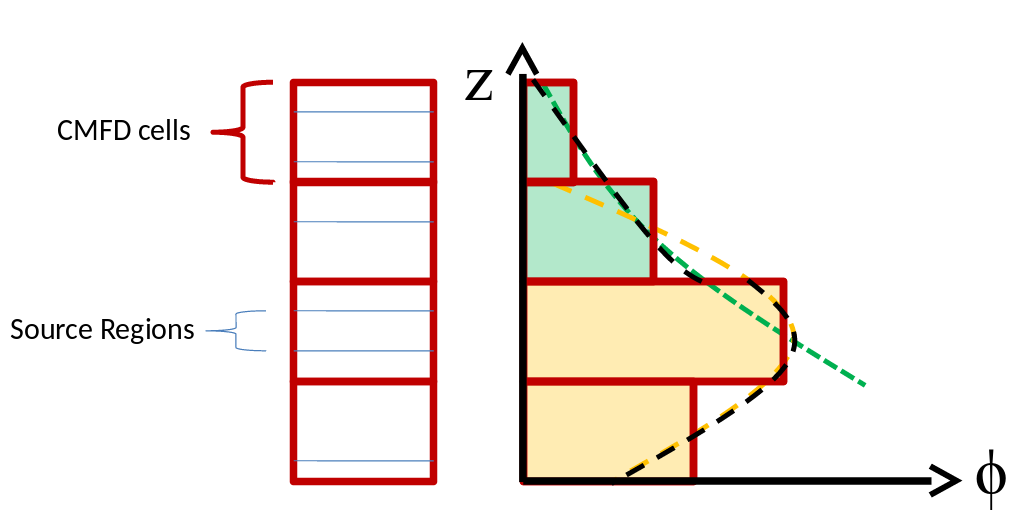
\includegraphics[width=\linewidth]{figures/axial-prolongation.png}
	\caption[]{A depiction of the axial prolongation for updating \ac{MOC} fluxes with \ac{CMFD} acceleration. The green dashed line shows the expansion in the top two axial \ac{CMFD} cells and the orange dashed line shows the expansion used in the bottom two \ac{CMFD} cells. The black dashed line shows the composite of the expansions.}
	\label{fig:axial-prolongation}
\end{figure}

\newpage

Updating the \ac{MOC} fluxes with the \ac{CMFD} solution allows convergence to be greatly accelerated, quickly capturing the flux shape over the coarse mesh. In addition, the computational cost of fully converging the \ac{CMFD} solution is small in comparison with just one \ac{MOC} transport sweep. Therefore, using the process laid out at the beginning of this chapter in Figure~\ref{fig:multigrid-cmfd}, the \ac{CMFD} equations are formed and solved after every transport sweep. This process for solving the \ac{MOC} neutron transport eigenvalue problem with \ac{CMFD} acceleration is detailed in Alg.~\ref{alg:moc-cmfd-eigenvalue-solve}.

\begin{algorithm}
	\caption[MOC Eigenvalue Solver with CMFD Acceleration]{MOC Eigenvalue Solver with CMFD Acceleration}
	\label{alg:moc-cmfd-eigenvalue-solve}
	\begin{algorithmic}[1]
		\Procedure{computeEigenvalue}{$geometry$, $tracks$, $N$}
		\State Implicitly define $F$, $S$, $H$, $D$, and $T$ from $geometry$ \Comment{Definitions in App.~\ref{app:matrix-moc}}
		\State $\boldsymbol{\phi} \gets \mathbb{1}$ \Comment{Initialize scalar fluxes to all ones}
		\State $\boldsymbol{\psi} \gets 0$ \Comment{\parbox[t]{.4\linewidth}{Initialize angular fluxes to zeros (only boundary stored)}}
		\State $k \gets 1$ \Comment{Initialize the eigenvalue to 1}
		\State $\boldsymbol{\phi} \gets \boldsymbol{\phi} \, / \, \left(\mathbb{1}^T F \boldsymbol{\phi}\right)$ \Comment{Normalize by total fission source}
		\While{not converged}
		\State $\mathbf{q} \gets \frac{1}{4\pi} \left(S \boldsymbol{\phi} + \frac{1}{k} F \boldsymbol{\phi} \right)$ \Comment{Compute neutron sources}
		\State \parbox[t]{.3\linewidth}{$\boldsymbol{\psi} \gets T^{-1} H D^{-1} \mathbf{q}$ \\ $\mathbf{p} \gets W \boldsymbol{\psi}$} \Comment{\parbox[t]{.5\linewidth}{Transport Sweep: these equations are solved simultaneously for computational efficiency. Currents on CMFD surfaces are tallied. Only angular fluxes on the boundary are explicitly stored.}}
		\State $\boldsymbol{\phi} \gets D^{-1}\mathbf{q} + D^{-1}
		\mathbf{p}$ \Comment{Scalar fluxes computed from tally $\mathbf{p}$}
		\State Form CMFD matrices $A$ and $M$ \Comment{\parbox[t]{.4\linewidth}{Defined by Eq.~\ref{eqn:cmfd_balance_grouped} and Eq.~\ref{eqn:cmfd_eigenvalue_problem} \\ (\textbf{restriction})}}
		\State Compute CMFD scalar fluxes $\Phi_C$ \Comment{Defined by Eq.~\ref{eqn:cmfd_scalar_fluxes} (\textbf{restriction})}
		\State $\Phi_C \gets \Phi_C \, / \, \left(\mathbb{1}^T M \Phi_C\right)$ \Comment{Normalize by total CMFD fission rate}
		\State $\tilde{\Phi}_C \gets \Phi_C$ \Comment{Save pre-CMFD scalar fluxes}
		\While{not converged}
		\State $\Phi_C \gets A^{-1} M \Phi_C$ \Comment{\parbox[t]{.5\linewidth}{Compute inverse with a linear solver \\ (Gauss-Seidel)}}
		\State $k \gets \mathbb{1}^T M \Phi_C$ \Comment{\parbox[t]{.5\linewidth}{Implicitly computing \\ $\left(\mathbb{1}^T M A^{-1} M \Phi_C\right) \, / \, \left(\mathbb{1}^T M \Phi_C\right)$}}
		\State $\Phi_C \gets \Phi_C \, / \, \left(\mathbb{1}^T M \Phi_C\right)$ \Comment{Normalize by total CMFD fission rate}
		\EndWhile
		\State \parbox[t]{.4\linewidth}{Update $\boldsymbol{\phi}$ by interpolating the \\ ratio of $\Phi_C$ and $\tilde{\Phi}_C$} \Comment{This is the \textbf{prolongation} step}
		\State $\boldsymbol{\phi} \gets \boldsymbol{\phi} \, / \, \left(\mathbb{1}^T F \boldsymbol{\phi}\right)$ \Comment{Normalize by total fission source}
		\EndWhile
		\State \textbf{return} $\boldsymbol{\phi}$ and $k$ \Comment{Return scalar fluxes and the eigenvalue}
		\EndProcedure
	\end{algorithmic}
\end{algorithm}

%%%%%%%%%%%%%%%%%%%%%%%%%%%%%%%%%%%%%%%%%%%%%%%%%%%%%%%%%%%%%%%%%%%%%%%%%%%%%%%
\chapter{Energy Group Structures}
\label{app:energy-groups}

The energy group structures are from the CASMO-4 lattice physics code~\cite{edenius1995casmo}.

\renewcommand{\arraystretch}{0.8}% Tighter

\begin{table}[h!]
  \centering
  \footnotesize
  \caption{One group energy boundaries.}
  \label{table:app-1-groups} 
  \vspace{14pt}
  \begin{tabular}{c r r}
    \toprule
    {\bf Group No.} &
    {\bf Lower Bound [MeV]} &
    {\bf Upper Bound [MeV]} \\
    \midrule
1 & 0.0000E+00 & 2.0000E+01 \\
    \bottomrule
   \end{tabular}
\end{table}

\begin{table}[h!]
  \centering
  \footnotesize
  \caption{Two group energy boundaries.}
  \label{table:app-2-groups} 
  \vspace{14pt}
  \begin{tabular}{c r r}
    \toprule
    {\bf Group No.} &
    {\bf Lower Bound [MeV]} &
    {\bf Upper Bound [MeV]} \\
    \midrule
2 & 0.0000E+00 & 6.2500E-07 \\
1 & 6.2500E-07 & 2.0000E+01 \\
  \bottomrule
 \end{tabular}
\end{table}

\begin{table}[h!]
  \centering
  \footnotesize
  \caption{Four group energy boundaries.}
  \label{table:app-4-groups} 
  \vspace{14pt}
  \begin{tabular}{c r r}
    \toprule
    {\bf Group No.} &
    {\bf Lower Bound [MeV]} &
    {\bf Upper Bound [MeV]} \\
    \midrule
4 & 0.0000E+00 & 6.2500E-07 \\
3 & 6.2500E-07 & 5.5300E-03 \\
2 & 5.5300E-03 & 8.2100E-01 \\
1 & 8.2100E-01 & 2.0000E+01 \\
  \bottomrule
 \end{tabular}
\end{table}

\begin{table}[h!]
  \centering
  \footnotesize
  \caption{Eight group energy boundaries.}
  \label{table:app-8-groups} 
  \vspace{14pt}
  \begin{tabular}{c r r}
    \toprule
    {\bf Group No.} &
    {\bf Lower Bound [MeV]} &
    {\bf Upper Bound [MeV]} \\
    \midrule
8 & 0.0000E+00 & 5.8000E-08 \\
7 & 5.8000E-08 & 1.4000E-07 \\
6 & 1.4000E-07 & 2.8000E-07 \\
5 & 2.8000E-07 & 6.2500E-07 \\
4 & 6.2500E-07 & 4.0000E-06 \\
3 & 4.0000E-06 & 5.5300E-03 \\
2 & 5.5300E-03 & 8.2100E-01 \\
1 & 8.2100E-01 & 2.0000E+01 \\
  \bottomrule
 \end{tabular}
\end{table}

\begin{table}[h!]
	\centering
	\footnotesize
	\caption{Eleven group energy boundaries.}
	\label{table:app-11-groups} 
	\vspace{14pt}
	\begin{tabular}{c r r}
		\toprule
		{\bf Group No.} &
		{\bf Lower Bound [MeV]} &
		{\bf Upper Bound [MeV]} \\
		\midrule
		11 & 0.0000E+00 & 5.8000E-08 \\
		10 & 5.8000E-08 & 1.4000E-07 \\
		9 & 1.4000E-07 & 2.8000E-07 \\
		8 & 2.8000E-07 & 6.2500E-07 \\
		7 & 6.2500E-07 & 4.0000E-06 \\
		6 & 4.0000E-06 & 9.8770E-06 \\
		5 & 9.8770E-06 & 1.5968E-05 \\
		4 & 1.5968E-05 & 2.7700E-05 \\
		3 & 2.7700E-05 & 5.5300E-03 \\
		2 & 5.5300E-03 & 8.2100E-01 \\
		1 & 8.2100E-01 & 2.0000E+01 \\
		\bottomrule
	\end{tabular}
\end{table}

\begin{table}[h!]
  \centering
  \footnotesize
  \caption{Sixteen group energy boundaries.}
  \label{table:app-16-groups} 
  \vspace{14pt}
  \begin{tabular}{c r r}
    \toprule
    {\bf Group No.} &
    {\bf Lower Bound [MeV]} &
    {\bf Upper Bound [MeV]} \\
    \midrule
16 & 0.0000E+00 & 3.0000E-08 \\
15 & 3.0000E-08 & 5.8000E-08 \\
14 & 5.8000E-08 & 1.4000E-07 \\
13 & 1.4000E-07 & 2.8000E-07 \\
12 & 2.8000E-07 & 3.5000E-07 \\
11 & 3.5000E-07 & 6.2500E-07 \\
10 & 6.2500E-07 & 8.5000E-07 \\
9 & 8.5000E-07 & 9.7200E-07 \\
8 & 9.7200E-07 & 1.0200E-06 \\
7 & 1.0200E-06 & 1.0970E-06 \\
6 & 1.0970E-06 & 1.1500E-06 \\
5 & 1.1500E-06 & 1.3000E-06 \\
4 & 1.3000E-06 & 4.0000E-06 \\
3 & 4.0000E-06 & 5.5300E-03 \\
2 & 5.5300E-03 & 8.2100E-01 \\
1 & 8.2100E-01 & 2.0000E+01 \\
  \bottomrule
 \end{tabular}
\end{table}

\begin{table}[h!]
  \centering
  \footnotesize
  \caption{Twenty-five group energy boundaries.}
  \label{table:app-25-groups} 
  \vspace{14pt}
  \begin{tabular}{c r r}
    \toprule
    {\bf Group No.} &
    {\bf Lower Bound [MeV]} &
    {\bf Upper Bound [MeV]} \\
    \midrule
25 & 0.0000E+00 & 3.0000E-08 \\
24 & 3.0000E-08 & 5.8000E-08 \\
23 & 5.8000E-08 & 1.4000E-07 \\
22 & 1.4000E-07 & 2.8000E-07 \\
21 & 2.8000E-07 & 3.5000E-07 \\
20 & 3.5000E-07 & 6.2500E-07 \\
19 & 6.2500E-07 & 9.7200E-07 \\
18 & 9.7200E-07 & 1.0200E-06 \\
17 & 1.0200E-06 & 1.0970E-06 \\
16 & 1.0970E-06 & 1.1500E-06 \\
15 & 1.1500E-06 & 1.8550E-06 \\
14 & 1.8550E-06 & 4.0000E-06 \\
13 & 4.0000E-06 & 9.8770E-06 \\
12 & 9.8770E-06 & 1.5968E-05 \\
11 & 1.5968E-05 & 1.4873E-04 \\
10 & 1.4873E-04 & 5.5300E-03 \\
9 & 5.5300E-03 & 9.1180E-03 \\
8 & 9.1180E-03 & 1.1100E-01 \\
7 & 1.1100E-01 & 5.0000E-01 \\
6 & 5.0000E-01 & 8.2100E-01 \\
5 & 8.2100E-01 & 1.3530E+00 \\
4 & 1.3530E+00 & 2.2310E+00 \\
3 & 2.2310E+00 & 3.6790E+00 \\
2 & 3.6790E+00 & 6.0655E+00 \\
1 & 6.0655E+00 & 2.0000E+01 \\
  \bottomrule
 \end{tabular}
\end{table}

\afterpage{
	\renewcommand*{\arraystretch}{0.6}% Tighter
	\footnotesize
	\begin{longtable}[h!]{c r r}
		\caption{Seventy group energy boundaries.} \\
		\label{table:app-70-groups} \\
		\toprule
		{\bf Group No.} &
		{\bf Lower Bound [MeV]} &
		{\bf Upper Bound [MeV]} \\
		\midrule
		70 & 0.0000E+00 & 5.0000E-09 \\
		69 & 5.0000E-09 & 1.0000E-08 \\
		68 & 1.0000E-08 & 1.5000E-08 \\
		67 & 1.5000E-08 & 2.0000E-08 \\
		66 & 2.0000E-08 & 2.5000E-08 \\
		65 & 2.5000E-08 & 3.0000E-08 \\
		64 & 3.0000E-08 & 3.5000E-08 \\
		63 & 3.5000E-08 & 4.2000E-08 \\
		62 & 4.2000E-08 & 5.0000E-08 \\
		61 & 5.0000E-08 & 5.8000E-08 \\
		60 & 5.8000E-08 & 6.7000E-08 \\
		59 & 6.7000E-08 & 8.0000E-08 \\
		58 & 8.0000E-08 & 1.0000E-07 \\
		57 & 1.0000E-07 & 1.4000E-07 \\
		56 & 1.4000E-07 & 1.8000E-07 \\
		55 & 1.8000E-07 & 2.2000E-07 \\
		54 & 2.2000E-07 & 2.5000E-07 \\
		53 & 2.5000E-07 & 2.8000E-07 \\
		52 & 2.8000E-07 & 3.0000E-07 \\
		51 & 3.0000E-07 & 3.2000E-07 \\
		50 & 3.2000E-07 & 3.5000E-07 \\
		49 & 3.5000E-07 & 4.0000E-07 \\
		48 & 4.0000E-07 & 5.0000E-07 \\
		47 & 5.0000E-07 & 6.2500E-07 \\
		46 & 6.2500E-07 & 7.8000E-07 \\
		45 & 7.8000E-07 & 8.5000E-07 \\
		44 & 8.5000E-07 & 9.1000E-07 \\
		43 & 9.1000E-07 & 9.5000E-07 \\
		42 & 9.5000E-07 & 9.7200E-07 \\
		41 & 9.7200E-07 & 9.9600E-07 \\
		40 & 9.9600E-07 & 1.0200E-06 \\
		39 & 1.0200E-06 & 1.0450E-06 \\
		38 & 1.0450E-06 & 1.0710E-06 \\
		37 & 1.0710E-06 & 1.0970E-06 \\
		36 & 1.0970E-06 & 1.1230E-06 \\
		35 & 1.1230E-06 & 1.1500E-06 \\
		34 & 1.1500E-06 & 1.3000E-06 \\
		33 & 1.3000E-06 & 1.5000E-06 \\
		32 & 1.5000E-06 & 1.8550E-06 \\
		31 & 1.8550E-06 & 2.1000E-06 \\
		30 & 2.1000E-06 & 2.6000E-06 \\
		29 & 2.6000E-06 & 3.3000E-06 \\
		28 & 3.3000E-06 & 4.0000E-06 \\
		27 & 4.0000E-06 & 9.8770E-06 \\
		26 & 9.8770E-06 & 1.5968E-05 \\
		25 & 1.5968E-05 & 2.7700E-05 \\
		24 & 2.7700E-05 & 4.8052E-05 \\
		23 & 4.8052E-05 & 7.5501E-05 \\
		22 & 7.5501E-05 & 1.4873E-04 \\
		21 & 1.4873E-04 & 3.6726E-04 \\
		20 & 3.6726E-04 & 9.0690E-04 \\
		19 & 9.0690E-04 & 1.4251E-03 \\
		18 & 1.4251E-03 & 2.2395E-03 \\
		17 & 2.2395E-03 & 3.5191E-03 \\
		16 & 3.5191E-03 & 5.5300E-03 \\
		15 & 5.5300E-03 & 9.1180E-03 \\
		14 & 9.1180E-03 & 1.5030E-02 \\
		13 & 1.5030E-02 & 2.4780E-02 \\
		12 & 2.4780E-02 & 4.0850E-02 \\
		11 & 4.0850E-02 & 6.7340E-02 \\
		10 & 6.7340E-02 & 1.1100E-01 \\
		9 & 1.1100E-01 & 1.8300E-01 \\
		8 & 1.8300E-01 & 3.0250E-01 \\
		7 & 3.0250E-01 & 5.0000E-01 \\
		6 & 5.0000E-01 & 8.2100E-01 \\
		5 & 8.2100E-01 & 1.3530E+00 \\
		4 & 1.3530E+00 & 2.2310E+00 \\
		3 & 2.2310E+00 & 3.6790E+00 \\
		2 & 3.6790E+00 & 6.0655E+00 \\
		1 & 6.0655E+00 & 2.0000E+01 \\
		\bottomrule
	\end{longtable}
}

\chapter{On-the-fly Ray Tracing by $z$-Stack}
\label{app:z-stack}

In Chapter~\ref{chap:ray-tracing}, on-the-fly ray tracing was introduced. In this appendix, the relationships formed for calculating segment crossings of a $z$-stack are more thoroughly explained.

Recall that all tracks in a $z$-stack have the same polar angle $\theta$, project onto the same 2D track, and are separated by a constant axial ray spacing $\delta z$. Therefore, the axial height $z_i$ of the $i^{\textit{th}}$ lowest track (starting from 0) can be given as a function of distance $s$ along the associated 2D track as
\begin{equation}
z_i(s) = z_0(0) + i\delta z + s \cot{\theta}
\label{eq::app-track_projection}
\end{equation}
where $z_0(0)$ is the $z$-coordinate at the intersection of the lowest track with the $z$-axis at the start of the associated 2D track.

For each 2D segment in the 2D track, there is an associated axially extruded region which contains a list of 3D \ac{SR}s in the region. Using the boundaries of each \ac{SR} and Eq.~\ref{eq::app-track_projection}, it is possible to analytically compute the indexes in the $z$-stack of tracks that will cross the \ac{SR}.

To begin, the first track to traverse the \ac{SR} (lowest index $i$) is determined. All tracks that traverse the \ac{SR} must have their highest $z$-height above the lowest boundary of the \ac{SR}, $z_{\textit{min}}$. Specifically,
\begin{equation}
\max_{s_{\textit{start}} \, \leq \, s \, \leq \, s_{\textit{end}}} z_i(s) > z_{\textit{min}}
\end{equation}
where $s_{\textit{start}}$ is the $s$ distance along the 2D track at the start of the 2D segment and $s_{\textit{end}}$ is the $s$ distance along the 2D track at the end of the 2D segment. Inserting the relationship in Eq.~\ref{eq::app-track_projection}, this can be expanded to
\begin{equation}
\max_{s_{\textit{start}} \, \leq \, s \, \leq \, s_{\textit{end}}} z_0(0) + i\delta z + s \cot{\theta} > z_{\textit{min}}.
\end{equation}
Noting the linear relationship of the tracks and the constant axial ray spacing, this can be simplified in terms of the lowest track with height $z_0$ as
\begin{equation}
\max\left(z_0(s_{\textit{start}}), z_0(s_{\textit{end}})\right) + i\delta z > z_{\textit{min}}
\end{equation}
and cast in terms of the index $i$ as
\begin{equation}
i > \frac{z_{\textit{min}} - \max\left(z_0(s_{\textit{start}}), z_0(s_{\textit{end}})\right)}{\delta z}.
\end{equation}
Since $i$ is an integer, the lowest track index $i_{\textit{start}}$ to traverse the region can be given by
\begin{equation}
i_{\textit{start}} = \Bigg\lceil\frac{z_{\textit{min}} - \max\left({z_0(s_{\textit{start}}), z_0(s_{\textit{end}})}\right) }{\delta z}\Bigg\rceil
\end{equation}

Next, the last track to traverse the \ac{SR} (highest index $i$) is determined. All tracks that traverse the \ac{SR} must have their lowest $z$-height below the highest boundary of the \ac{SR}, $z_{\textit{max}}$. Specifically,
\begin{equation}
\min_{s_{\textit{start}} \, \leq \, s \, \leq \, s_{\textit{end}}} z_i(s) < z_{\textit{max}}
\end{equation}
which can be expanded to
\begin{equation}
\min_{s_{\textit{start}} \, \leq \, s \, \leq \, s_{\textit{end}}} z_0(0) + i\delta z + s \cot{\theta} < z_{\textit{max}}.
\end{equation}
Similar to the arguments for the first track index, the last track index follows the criteria
\begin{equation}
i < \frac{z_{\textit{max}} - \min\left(z_0(s_{\textit{start}}), z_0(s_{\textit{end}})\right)}{\delta z}.
\end{equation}
Therefore, the last track to cross the \ac{SR} has index $i_{\textit{end}}$ given by
\begin{equation}
i_{\textit{end}} = \Bigg\lfloor\frac{z_{\textit{max}} - \min\left({z_0(s_{\textit{start}}), z_0(s_{\textit{end}})}\right) }{\delta z}\Bigg\rfloor.
\end{equation}

In addition to analytically calculating the first and last track indexes, it is possible to calculate the indexes of tracks with the same length. Specifically, it is possible to calculate the first and last tracks to cross the entire 2D segment length or the entire 3D source height.

For a track to cross the entire 2D segment length, both its beginning and ending heights must be between the minimum and maximum \ac{SR} boundaries. For a track to cross the entire axial height of the \ac{SR}, its beginning and ending heights must be above and below the minimum and maximum \ac{SR} boundaries, respectively.

Two indexes $i_{\textit{in}}$ and $i_{\textit{out}}$ are calculated. The index $i_{\textit{in}}$ represents the first track to start above the lowest \ac{SR} boundary and $i_{\textit{out}}$ represents the first track to end above the maximum \ac{SR} boundary. All tracks with index between $i_{\textit{in}}$ and $i_{\textit{out}}$ traverse the entire 2D segment length. All tracks with index between $i_{\textit{out}}$ and $i_{\textit{in}}$ will traverse the entire \ac{SR} height. Notice that these are mutually exclusive: if some tracks traverse the entire 2D segment length, none will traverse the entire \ac{SR} height.

Tracks that start above the minimum boundary satisfy
\begin{equation}
\min_{s_{\textit{start}} \, \leq \, s \, \leq \, s_{\textit{end}}} z_i(s) > z_{\textit{min}}
\end{equation}
and tracks that end above the maximum boundary satisfy
\begin{equation}
\max_{s_{\textit{start}} \, \leq \, s \, \leq \, s_{\textit{end}}} z_i(s) > z_{\textit{max}}.
\end{equation}
Therefore, in a similar process to determining the first and last tracks to cross the \ac{SR}, the indexes $i_{\textit{in}}$ and $i_{\textit{out}}$ can be calculated as:
\begin{equation}
i_{\textit{in}} = \Bigg\lceil\frac{z_{\textit{min}} - \min\left({z_0(s_{\textit{start}}), z_0(s_{\textit{end}}})\right) }{\delta z}\Bigg\rceil
\end{equation}
\begin{equation}
i_{\textit{out}} = \Bigg\lceil\frac{z_{\textit{max}} - \max\left({z_0(s_{\textit{start}}), z_0(s_{\textit{end}}})\right) }{\delta z}\Bigg\rceil
\end{equation}

\chapter{The BEAVRS Benchmark}
\label{chap:beavrs}

The main results presented in this thesis are based on models formed from the BEAVRS benchmark~\cite{horelik2013beavrs}. This chapter introduces the BEAVRS benchmark in Section~\ref{sec:beavrs-intro}, including a description of alteration made to the benchmark. Section~\ref{sec:beavrs-xs-gen} describes how cross-sections are generated for the benchmark. Finally, Section~\ref{sec:beavrs-models} details the particular models formed from cutouts of the BEAVRS model and, in some cases, replication of the cutouts.

%%%%%%%%%%%%%%%%%%%%%%%%%%%%%%%%%%%%%%%%%%%%%%%%%%%%%%%%%%%%%%%%%%%%%%%%%%%%%%%%
\section{Introduction to the BEAVRS Benchmark}
\label{sec:beavrs-intro}

The BEAVRS benchmark~\cite{horelik2013beavrs} was released in 2013, representing a Westinghouse 4-loop nuclear power reactor. This reactor is representative of common \ac{PWR} designs in the United States. The benchmark contains core loadings and detector measurements for the first two cycles of operation, but this thesis concentrates on \ac{HZP} simulations at the beginning of the first cycle in an all rods out configuration.

The reactor contains 193 fuel assemblies. Each assembly contains a $17 \times 17$ lattice of fuel rods, guide tubes, and instrument tubes. The pin-pitch is 1.26 cm inside each assembly. All fuel rods within the same assembly contain uranium of the same enrichment. In the first cycle, three uranium enrichments are used: 1.6\%, 2.4\%, and 3.1\%. Wet annular burnable absorbers are present throughout the core to flatten the power distribution. The active fuel height is 365.76 cm. A radial description of the core is shown in Figure~\ref{fig:beavrs-assembly-enrichment}.

\begin{figure}[h!]
	\centering
	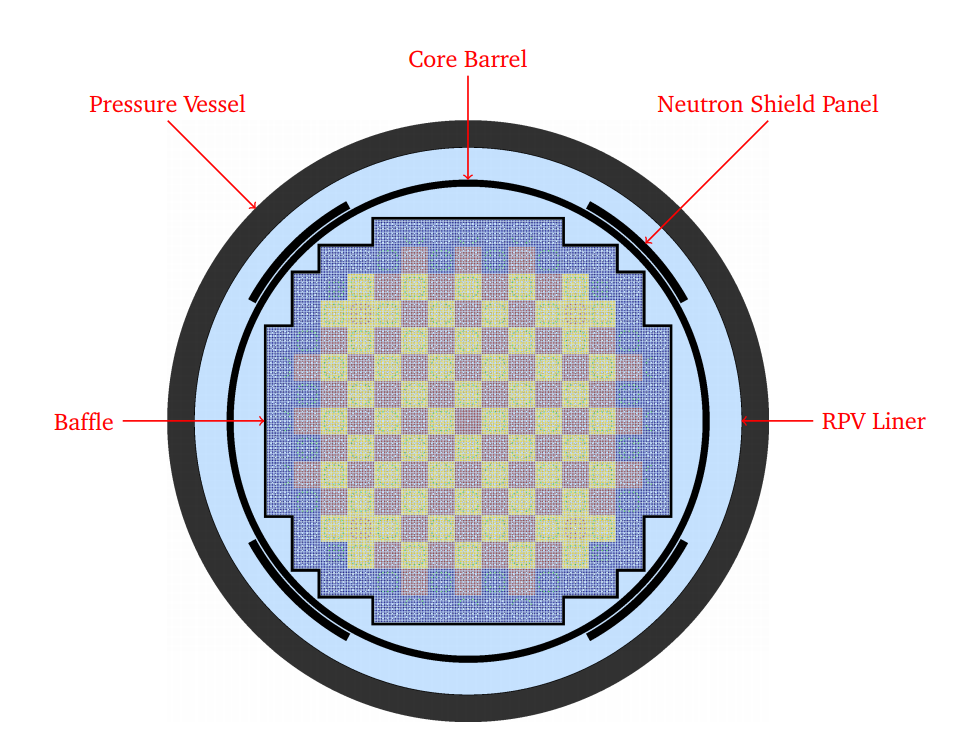
\includegraphics[width=\linewidth]{figures/beavrs-visual/beavrs-assembly-enrichment.png}
	\caption{A radial illustration of the BEAVRS benchmark with fuel pins colored by enrichment.}
	\label{fig:beavrs-assembly-enrichment}
\end{figure} 

The goal of this thesis is to simulate the BEAVRS benchmark using the explicit detail provided in the BEAVRS specification. However, in order to conduct uniform axial mesh refinement studies, the axial heights of material regions are altered such that each discontinuity occurs at an even number (in cm). The top and bottom grid spacers in the BEAVRS benchmark were defined to be 5.72 cm with intermediate grid spacers 3.36 cm. These lengths were altered to 6.0 cm and 2.0 cm respectively. The starting height of the grid spacers were rounded to the nearest even integer. All other $z$-heights in the geometry were similarly rounded to the nearest integer. The altering of axial heights allows regions to be formed which all have the same axial height, which can simplify sensitivity analysis. While these alterations do change the benchmark slightly -- and therefore also change the computed solutions -- these solutions are still representative of a realistic \ac{PWR} problem.

Although the BEAVRS model is defined inside a cylindrical geometry, a rectangular bounding geometry is often necessary in \ac{MOC} methods for cyclic tracking. Therefore, the BEAVRS model is modeled with a rectangular prism bounding the geometry. In the radial plane, the bounding dimensions are square with length equal to 17 assembly widths. Since the BEAVRS model has a maximum of 15 assemblies along each $x$ and $y$ direction, this allows at least one assembly of radial reflector to be modeled outside the core. In addition, the corners have very deep water reflectors. In the axial direction, the BEAVRS benchmark is modeled with 400 cm height, allowing approximately 20 cm of axial reflector in each direction. Vacuum boundaries are assumed on all surfaces. 


%%%%%%%%%%%%%%%%%%%%%%%%%%%%%%%%%%%%%%%%%%%%%%%%%%%%%%%%%%%%%%%%%%%%%%%%%%%%%%%%
\section{Cross-Section Generation}
\label{sec:beavrs-xs-gen}

In this thesis, the same 70 group cross-section library is used for all results involving the BEAVRS benchmark or cutouts of the BEAVRS benchmark except for the rod insertion studies. A separate 70 group cross-section library was formed for rod insertion studies in order to form accurate cross-sections for control rod materials. In this section, the process used to form cross-sections is thoroughly discussed.

Using the OpenMC Monte Carlo code, reaction rate tallies are generated for each unique material. These allow for the computation of multi-group cross-sections with the methodology discussed in Chapter~\ref{chap:mgxs} using the \texttt{mgxs} package implemented by Boyd~\cite{boyd2017thesis}. The 70 group library is formed from an OpenMC simulation of the full core BEAVRS benchmark. The Monte Carlo simulation used 400 batches (300 inactive, 100 active) with $2 \times 10^8$ particles per batch. The in-scatter transport correction described in Section~\ref{sec:transport-correction} is applied to the cross-sections using anisotropic scattering tallies. Note that using these tallies to form the transport correction introduces approximation since the true tallies should involve angular fluxes rather than scalar fluxes. Since the anisotropic current tallies could vary significantly between core and outer reflector regions, the water is split into two materials for which cross-sections are independently formed: core water and outer reflector water. In addition, a third water material is also formed near the support plate nozzle as the isotopic composition differs due to boron concentration. A plot of the BEAVRS benchmark colored by unique material region is shown in Figure~\ref{fig:beavrs-materials-radial}. In addition an axial plot of the materials is shown in Figure~\ref{fig:beavrs-materials-axial}. Similarly the radial and axial material plots of a 1.6\% enriched fuel assembly are shown in Figure~\ref{fig:beavrs-single-assembly-materials-radial} and Figure~\ref{fig:beavrs-single-assembly-materials-axial}, respectively.


\begin{figure}[h!]
	\centering
	\includegraphics[width=\linewidth]{figures/beavrs-visual/materials-beavrs-radial.jpg}
	\caption{A radial view of the BEAVRS benchmark with regions colored by material.}
	\label{fig:beavrs-materials-radial}
\end{figure} 

\begin{figure}[h!]
	\centering
	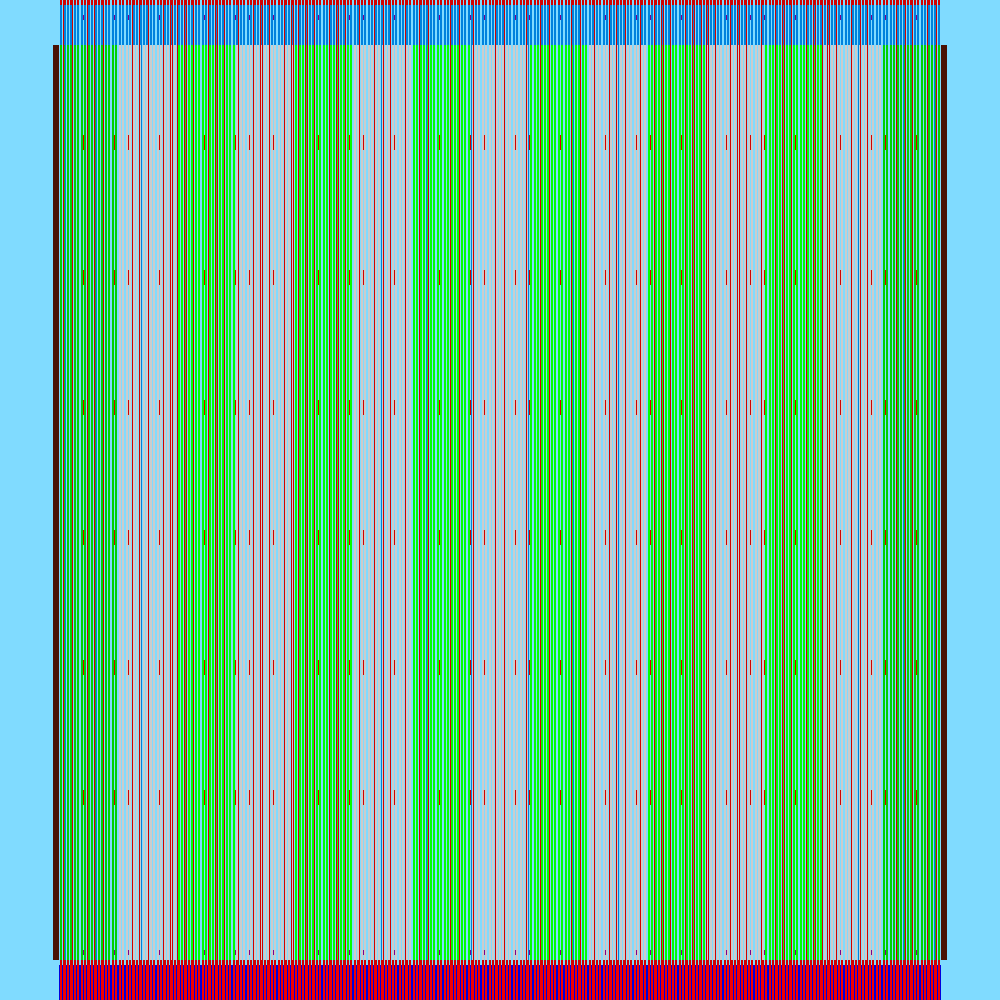
\includegraphics[width=\linewidth]{figures/beavrs-visual/materials-beavrs-axial.jpg}
	\caption{An axial view of the BEAVRS benchmark with regions colored by material.}
	\label{fig:beavrs-materials-axial}
\end{figure} 

\begin{figure}[h!]
	\centering
	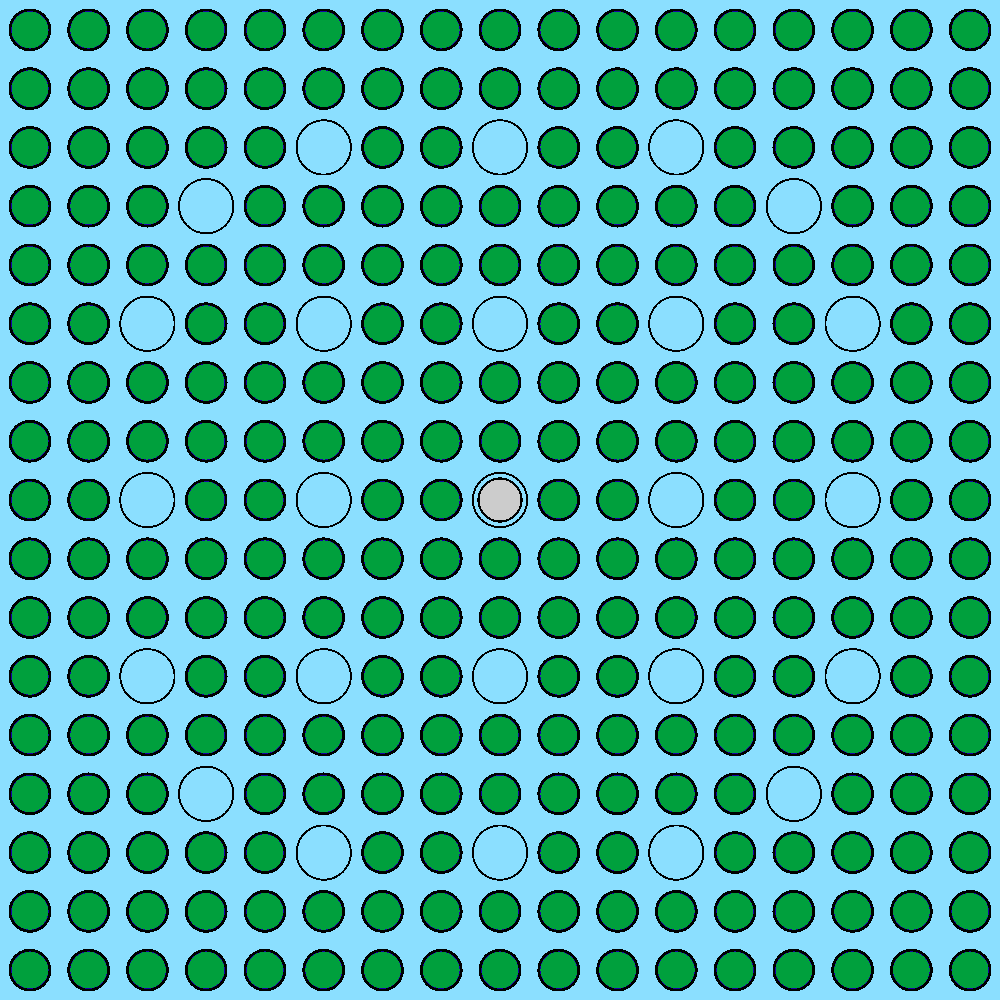
\includegraphics[width=0.65\linewidth]{figures/beavrs-visual/materials-single-assembly-radial.png}
	\caption{A radial view of the 1.6\% enriched fuel assembly in the BEAVRS benchmark with regions colored by material.}
	\label{fig:beavrs-single-assembly-materials-radial}
\end{figure} 

\begin{figure}[h!]
	\centering
	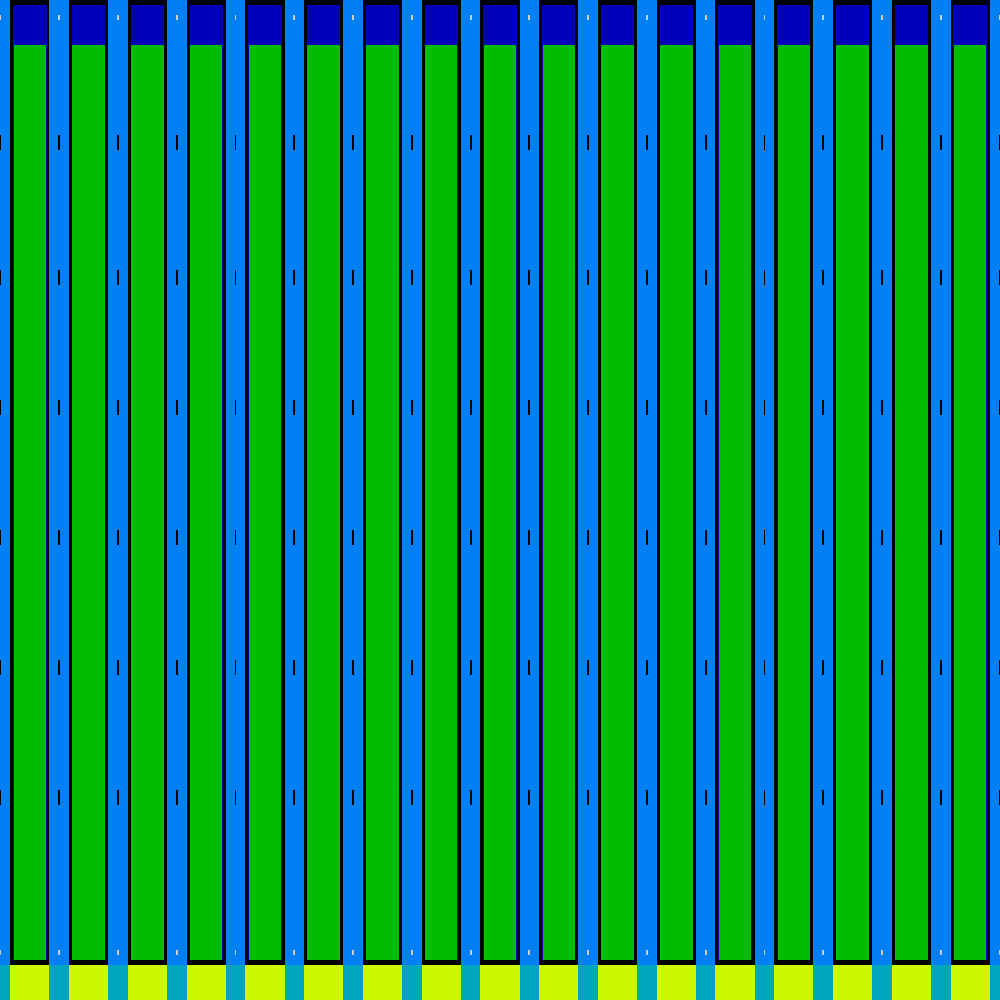
\includegraphics[width=0.65\linewidth]{figures/beavrs-visual/materials-single-assembly-axial.png}
	\caption{An axial view of 1.6\% enriched fuel assembly in the BEAVRS benchmark with regions colored by material.}
	\label{fig:beavrs-single-assembly-materials-axial}
\end{figure} 



\clearpage

The computed cross-sections were compared with CASMO-4 cross-sections and significant differences were found in the transport correction for water. In preliminary tests, the CASMO-4 multi-group cross-sections for core water were also able to much more accurately simulate the gross fission distribution. Therefore, instead of solely using the OpenMC \texttt{mgxs} cross-sections for core water which had an inaccurate transport correction, or solely using CASMO-4 cross-sections which are generated for more general problems, a new cross-section set was formed specifically for core water. Since CASMO-4 is a lattice physics code, it is designed to have accurate estimates of core water cross-sections. Therefore, the transport correction from CASMO-4 is used to modify the cross-sections formed by the OpenMC \texttt{mgxs} package. Specifically, the transport cross-section $\Sigma_{tr}^g$ for group $g$ is formed by computing
\begin{equation}
\Sigma_{tr}^g = \Sigma_{a}^g + \eta \left( \Sigma_{t}^g - \Sigma_{a}^g \right)
\end{equation}
where $\Sigma_{a}^g$ and $\Sigma_{t}^g$ are the associated absorption and total cross-sections formed by \texttt{mgxs}, respectively. The factor $\eta$ is computed by
\begin{equation}
\eta = \frac{\Sigma_{tr}^{g, \textbf{CASMO}} - \Sigma_{a}^{g, \textbf{CASMO}}}{\Sigma_{t}^{g, \textbf{CASMO}} - \Sigma_{a}^{g, \textbf{CASMO}}}
\end{equation}
where the \textbf{CASMO} superscript denotes CASMO-4 cross-sections. It is important to note that this is only done for core water. All other materials use the cross-sections formed directly from the \texttt{mgxs} package in OpenMC.

%%%%%%%%%%%%%%%%%%%%%%%%%%%%%%%%%%%%%%%%%%%%%%%%%%%%%%%%%%%%%%%%%%%%%%%%%%%%%%%%
\section{Description of BEAVRS Models}
\label{sec:beavrs-models}

All models which are simulated in this thesis are derived from cutouts of the BEAVRS benchmark with 70 group cross-sections. In past presentations the, 3D \ac{MOC} solver implemented in this thesis has been verified on a variety of simpler, conventional reactor physics models~\cite{physor2016shaner, physor2016otf}. The BEAVRS benchmark represents a far more computationally demanding challenge, especially with a 70 group cross-section library. Cutouts are formed in order to evaluate smaller problems which are representative of computational performance or physical behavior of the large full core problem.

\subsection{Full Core 3D Model}
\label{sec:beavrs-3D}

The first model is just the BEAVRS model incorporating all the details discussed in previous sections. The simulation of this model directly corresponds with the OpenMC simulations from which the cross-sections are derived. The objective of this thesis is to accurately simulate this model. However, due to the large computational cost of simulating this model, only minimal tests can be conducted. Therefore, smaller cutouts are formed which are more computationally feasible in order to test computational and physical behavior before running the 3D full core case.


\subsection{Full Core 2D Model}
\label{sec:beavrs-2D}

A 2D extruded cutout of the reactor is formed in order to determine the physical behavior of the BEAVRS model in the radial direction. This cutout is taken from an 10 cm axial interval over which there are no grid spacers. Reflective boundary conditions are placed on the top and bottom of the problem. While this model lacks any axial variation, it still contains all radial detail. Due to the lack of axial detail, 2D \ac{MOC} and 3D \ac{MOC} simulations with sufficient parameter refinement should produce equivalent solutions. Only this model and the full core 3D model contain the full radial water reflector. Therefore, this model is very useful in determining the effect of large radial water reflectors. 

\subsection{Single Assembly Model}
\label{sec:beavrs-single-assembly}

A single assembly model is formed which represents the full axial detail of a single 1.6\% enriched fuel assembly. While this model lacks radial water reflectors, it contains the full axial detail fo the full core problem, including grid spacers. Outside the core, full geometrical detail is also captured including support plate nozzles and, most notably, water reflectors of approximately 20 cm above and below the fuel. Reflective boundaries are placed on the $x$ and $y$ boundaries. Physically, this is equivalent to an infinite 2D lattice of 1.6\% enriched fuel assemblies. Vacuum boundaries remain on the top and bottom of this model. Since this problem is significantly less computationally expensive than the full core models (both 2D and 3D), it allows rigorous parameter refinement and convergence studies.

\subsection{Truncated Single Assembly Model}
\label{sec:trunc-single-assembly}

In addition to the single assembly model, a truncated single assembly model is also formed which contains all the detail of the single assembly model, but without the axial water reflectors. Specifically, 20 cm are removed from both the bottom and top of the model, resulting in a model that only covers the active fuel and is 360 cm tall. Axial boundaries still have vacuum boundary conditions. Comparison with the single assembly model described in Section~\ref{sec:beavrs-single-assembly} allows for the effect of axial water reflectors to be directly tested.

\subsection{SDSA Model}
\label{sec:sdsa}

The Single Domain Single Assembly (SDSA) model is formed for rigorous performance testing. It represents a 20 cm tall cutout within the single assembly model which contains no grid spacers. Reflective boundary conditions are imposed on all surfaces. Since this problem is far reduced in size, it allows for rigorous performance testing. In Chapter~\ref{chap:domain-decomposition}, spatial domain decomposition is introduced in which the geometry is split into equal sized domains in which each computational node is expected to handle one domain. When simulating the BEAVRS benchmark with domain decomposition, the expected domain size is the size of the SDSA model. Therefore, this model allows for realistic on-node performance characterization of the BEAVRS benchmark without needing to run the large full core problem.

\subsection{Short Single Assembly Model}
\label{sec:short-single-assembly}

Similar to the SDSA model, a short single assembly model is created which allows for studies at far reduced computational cost. This model is the same as the SDSA model except it is only 10 cm in axial height and contains 3.1\% enriched fuel. This enrichment is the highest enrichment found in the cycle 1 BEAVRS model. The higher enriched fuel allows for slightly larger gradients with a flux peak in the moderator. The primary focus of this model is to test in-core radial mesh sensitivity.


\subsection{Rodded Single Assembly Model}
\label{sec:rodded-single-assembly}

The rodded single assembly model is the only model which uses a geometry not explicitly found in the full core 3D BEAVRS model. The model is constructed in the same way as the single assembly model described in Section~\ref{sec:beavrs-single-assembly}, but with 3.1\% enriched fuel and with all rods inserted at 100 steps -- covering approximately half of the active fuel height. This large control rod insertion causes significant gradients within the axial scalar flux distribution, allowing for robust testing of 3D \ac{MOC} on problems with significant axial variation.

As mentioned previously, this model uses a separate cross-section library. Instead of simulating the all rods out configuration, which lacks control rods within the core, the single assembly model is explicitly simulated in OpenMC to form cross-section estimates. This allows reasonable estimates of control rod material cross-sections.


\newpage
\vfill
\begin{highlightsbox}[frametitle=Highlights]
	\begin{itemize}
		\item The BEAVRS benchmark represents a traditional \ac{PWR} reactor encompassing all relevant radial and axial detail
		\item The BEAVRS model is simulated within a radially square bounding box, leading to large corner reflector regions
		\item A 70 group cross-section library is formed through direct simulation of the BEAVRS benchmark in Monte Carlo using the OpenMC \texttt{mgxs} package with a combination of CASMO-4 and in-scatter transport corrections
		\item Cutouts of the BEAVRS model allow for physics and computational behavior to be tested with much lower computational cost
		\item A rodded single assembly model is created to test the effect of large axial variation, for which a separate cross-section library is generated in order to accurately capture control rod properties
		
	\end{itemize}
\end{highlightsbox}
\vfill



\chapter{Cross-section Generation}
\label{app:cross-section-gen}

In this thesis, the same 70 group cross-section library is used for all results involving the BEAVRS benchmark or cutouts of the BEAVRS benchmark, except for rod insertion studies in which a separate 70 group cross-section library was formed in order to have accurate control rod material cross-sections. All cross-section libraries and group structures use the CASMO-4 energy group boundaries~\cite{edenius1995casmo}, as given in Appendix~\ref{app:energy-groups}. In this appendix, the process used to form cross-sections is thoroughly discussed.

This appendix is split into four sections. First, the basics of multi-group cross-section generation are discussed in Section~\ref{sec:xs-generation}. Then the subtleties of angular dependence of total cross-sections and the formation of transport-corrected cross-sections are discussed in Section~\ref{sec:mgxs-angular-dependence} and Section~\ref{app:transport-correction}, respectively. Finally, the process to generate cross-sections using OpenMC is discussed in Section~\ref{sec:openmc-xs}


\section{Cross-section Generation}
\label{sec:xs-generation}

The multi-group transport equation yields solutions equivalent to those from the continuous energy transport equation if cross-sections are appropriately defined. This is obtained for a given energy group $g$ by integrating the continuous energy transport equation over the associated energy range of $[E_{g}, E_{g-1}]$. The resulting multi-group cross-section definitions are:
\begin{eqnarray}
\Sigma_{t}^g(\mathbf{r},\mathbf{\Omega}) = \frac{\int_{E_{g}}^{E_{g-1}} dE \, \Sigma_{t}(\mathbf{r},E)\psi(\mathbf{r},\mathbf{\Omega},E)}{\int_{E_{g}}^{E_{g-1}} dE \, \psi(\mathbf{r},\mathbf{\Omega},E)} 
\label{eqn:multi-group-xs-definitions-first}\\
\nu \Sigma_f^g\left(\mathbf{r}\right) = \frac{\int\displaylimits_{E_{g'}}^{E_{g'-1}} dE \, \nu(\mathbf{r},E) \Sigma_f(\mathbf{r}, E) \phi(\mathbf{r}, E)}{\int\displaylimits_{E_{g'}}^{E_{g'-1}} dE \, \phi(\mathbf{r}, E)} \\
\chi_g\left(\mathbf{r}\right) = \frac{\int\displaylimits_{E_{g'}}^{E_{g'-1}} dE \, \chi(\mathbf{r},E) \sum_{g'=1}^G \nu \Sigma_f^{g'}(\mathbf{r}) \phi_{g'}(\mathbf{r})}{\sum_{g=1}^G \nu \Sigma_f^{g}(\mathbf{r}) \phi_{g}(\mathbf{r})}
\end{eqnarray}
\begin{equation}
\begin{split}
\Sigma_{s}^{g' \rightarrow g}\left(\mathbf{r}\right) = \frac{\int_{E_{g}}^{E_{g-1}} dE \, \int\displaylimits_{E_{g'}}^{E_{g'-1}} dE' \,  \Sigma_{s}(\mathbf{r},{E'\rightarrow E}) \phi(\mathbf{r}, E') }{\int_{E_{g}}^{E_{g-1}} dE \, \phi(\mathbf{r},E)}
\end{split}
\label{eqn:multi-group-xs-definitions-last}
\end{equation}
While seemingly straightforward, these equations require knowledge of the neutron fluxes, which are the goal of transport simulations. Therefore, approximations need to be made for the fluxes. One way to implicitly do this is through Monte Carlo simulations in which reaction rates are tallied. These tallied reaction rates can be used in conjunction with a tallied scalar flux estimate to produce multi-group cross-sections.

\section{Angular Dependence of Total Cross-Sections}
\label{sec:mgxs-angular-dependence}

From the definition of the multi-group total cross section $\Sigma_{t}^g$ in Eq.~\ref{eqn:multi-group-xs-definitions-first} as 
\begin{equation}
\nonumber
\Sigma_{t}^g(\mathbf{r},\mathbf{\Omega}) = \frac{\int_{E_{g}}^{E_{g-1}} dE \, \Sigma_{t}(\mathbf{r},E)\psi(\mathbf{r},\mathbf{\Omega},E)}{\int_{E_{g}}^{E_{g-1}} dE \, \psi(\mathbf{r},\mathbf{\Omega},E)} ,
\end{equation}
it is clear that the multi-group total cross-section should be angular dependent even though we assume the continuous energy total cross-section is angular independent. This is because the total cross-section multiplies the angular flux rather than the scalar flux. In turn, this causes its collapsed multi-group form to be angular dependent since both the numerator and denominator of the expression in Eq.~\ref{eqn:multi-group-xs-definitions-first} are angular dependent. This would be true of any cross-section that multiplies the angular flux, but with the isotropic scattering approximation, there are no other terms that multiply cross-sections by the angular flux.

This angular dependence is often neglected, but can introduce a bias~\cite{gibson-preprint}. With the angular dependence ignored, the relationship can be integrated over all directions leading to the form in Eq.~\ref{eqn:tot-mgxs-sf}.
\begin{equation}
\Sigma_{t}^g(\mathbf{r}) = \frac{\int_{E_{g}}^{E_{g-1}} dE \, \Sigma_{t}(\mathbf{r},E)\phi(\mathbf{r},E)}{\int_{E_{g}}^{E_{g-1}} dE \, \phi(\mathbf{r},E)} 
\label{eqn:tot-mgxs-sf}
\end{equation}
The work in this thesis also relies on the approximation of angular independent multi-group total cross-sections. With this approximation, the new multi-group transport equation can be formed, as given in Eq.~\ref{eqn:multi-group-transport-2} whose solution is the subject of this thesis. 
\begin{equation}
\mathbf{\Omega} \cdot \nabla \psi_{g}(\mathbf{r},\mathbf{\Omega}) + \Sigma_t^{g}(\mathbf{r}) \psi_{g}(\mathbf{r},\mathbf{\Omega}) = \frac{1}{4 \pi} \left( \frac{\chi_{g}\left(\mathbf{r}\right)}{k} \sum_{g'=1}^{G} \nu_{g'}\left(\mathbf{r}\right) \Sigma_f^{g'}\left(\mathbf{r}\right) \phi_{g'}\left(\mathbf{r}\right) + \, \sum_{g'=1}^G \,  \Sigma_{s}^{g' \rightarrow g}\left(\mathbf{r}\right) \phi_{g'}(\mathbf{r}) \right)
\label{eqn:multi-group-transport-2}
\end{equation}
It is important to remember that some error is expected from the absence of angular dependent total cross-sections so that the multi-group transport solution does not strictly match the corresponding continuous energy transport solution, such as that computed by Monte Carlo methods.

\section{The Transport Correction}
\label{app:transport-correction}

Previously it was mentioned that the assumption of isotropic scattering introduces significant bias, but is remedied by a transport correction. In this section, the transport correction is derived and its implications are discussed. Many different transport corrections have been implemented, such as those described in the TRANSX~\cite{macfarlane1993transx} and NJOY~\cite{macfarlane2000njoy} manuals. The basis for these transport corrections was formulated by Bell, Hansen and Sandmeier~\cite{bell1967transport}. However, this section largely follows Hebert's derivation~\cite{hebert2009applied}. 

The scattering term, without the isotropic assumption, follows the relationship
\begin{equation}
	\int\displaylimits_{0}^{\infty} dE' \, \int\displaylimits_{4\pi} \, d\mathbf{\Omega'} \Sigma_{s}(\mathbf{r}, \mathbf{\Omega'}\rightarrow \mathbf{\Omega},{E'\rightarrow E}) \psi(\mathbf{r}, \mathbf{\Omega'},E').
	\label{eqn:xs-angular-dependence-removal}
\end{equation}
In the laboratory system, in which neutron behavior is modeled, scattering may be strongly anisotropic. However, in the center-of-momentum framework, scattering is nearly isotropic in the energy range of interest. This implies that the angular dependence relies on the magnitude of the deflection from scattering $\mathbf{\Omega} \cdot \mathbf{\Omega'}$, reducing this relationship to
\begin{equation*}
	\int\displaylimits_{0}^{\infty} dE' \, \int\displaylimits_{4\pi} \, d\mathbf{\Omega'} \Sigma_{s}(\mathbf{r}, \mathbf{\Omega} \cdot \mathbf{\Omega'},{E'\rightarrow E}) \psi(\mathbf{r}, \mathbf{\Omega'},E').
\end{equation*}
The scattering kernel can be expressed as an expansion of Legendre polynomials $P_\ell$ with angular-independent coefficients $\Sigma_{s,\ell}\left(\mathbf{r}, E'\rightarrow E \right)$ as shown in Eq.~\ref{eqn:scattering-expansion} where $\mu = \mathbf{\Omega} \cdot \mathbf{\Omega'}$.
\begin{equation}
\Sigma_{s}(\mathbf{r}, \mu,{E'\rightarrow E}) = \sum_{\ell=0}^\infty \frac{2 \ell + 1}{2} \Sigma_{s,\ell}\left(\mathbf{r}, E'\rightarrow E \right) P_\ell(\mu)
\label{eqn:scattering-expansion}
\end{equation}
The coefficients can be determined by taking advantage of the orthogonality of Legendre polynomials, leading to the relationship in Eq.~\ref{eqn:scattering-expansion-coefficients}.
\begin{equation}
\Sigma_{s,\ell}\left(\mathbf{r}, E'\rightarrow E \right) = \int_{-1}^{1} d\mu \, \Sigma_{s}(\mathbf{r}, \mu, {E'\rightarrow E}) P_\ell(\mu)
\label{eqn:scattering-expansion-coefficients}
\end{equation}
The scattering kernel can be approximated by a finite number $L$ of Legendre polynomials with modified coefficients $\tilde{\Sigma}_{s,\ell}\left(\mathbf{r}, E'\rightarrow E \right)$ and a transport correction term $\Delta \Sigma_{\textit{tr}}\left(\mathbf{r}, E'\rightarrow E \right)$ in Eq.~\ref{eqn:scattering-expansion-approx}.
\begin{equation}
\Sigma_{s}(\mathbf{r}, \mu, {E'\rightarrow E}) \approx \sum_{\ell=0}^L \frac{2 \ell + 1}{2} \tilde{\Sigma}_{s,\ell}\left(\mathbf{r}, E'\rightarrow E \right) P_\ell(\mu) + \Delta \Sigma_{\textit{tr}}\left(\mathbf{r}, E'\rightarrow E \right) \delta\left(\mu - 1\right)
\label{eqn:scattering-expansion-approx}
\end{equation}
Here $\delta$ represents the Dirac delta function, whose application to the transport correction makes the term forward peaked in the direction of travel to capture higher order anisotropies. Taking advantage of the relationship in Eq.~\ref{eqn:scattering-expansion-coefficients} and the approximation of the scattering kernel in Eq.~\ref{eqn:scattering-expansion-approx}, the true Legendre polynomial scattering coefficients can be related to the modified coefficients in Eq.~\ref{eqn:scattering-expansion-coefficients-approx}
\begin{equation}
\begin{split}
\Sigma_{s,\ell}\left(\mathbf{r}, E'\rightarrow E \right) \approx \int_{-1}^{1} d\mu \, \sum_{\ell'=0}^L \frac{2 \ell' + 1}{2} \tilde{\Sigma}_{s,\ell'}\left(\mathbf{r}, E'\rightarrow E \right) P_{\ell'}(\mu) P_\ell(\mu) \\ + \int_{-1}^{1} d\mu \, \Delta \Sigma_{\textit{tr}}\left(\mathbf{r}, E'\rightarrow E \right) \delta\left(\mu - 1\right) P_\ell(\mu)
\label{eqn:scattering-expansion-coefficients-approx}
\end{split}
\end{equation}
For $0 \leq \ell \leq L$, Eq.~\ref{eqn:scattering-expansion-coefficients-approx} can be simplified using the orthogonality of Legendre polynomials and the property $P_\ell(1) = 1$. This leads to the simplified relationship in Eq.~\ref{eqn:tc-simplified-coefficients}.
\begin{equation}
\Sigma_{s,\ell}\left(\mathbf{r}, E'\rightarrow E \right) \approx  \tilde{\Sigma}_{s,\ell}\left(\mathbf{r}, E'\rightarrow E \right) + \Delta \Sigma_{\textit{tr}}\left(\mathbf{r}, E'\rightarrow E \right)
\label{eqn:tc-simplified-coefficients}
\end{equation}
In order to capture the next order scattering after $L$, the transport correction term is set to capture scattering of order $L+1$ as shown in Eq.~\ref{eqn:tc-scattering-order}.
\begin{equation}
\Delta \Sigma_{\textit{tr}}\left(\mathbf{r}, E'\rightarrow E \right) = \Sigma_{s,L+1}\left(\mathbf{r}, E'\rightarrow E \right)
\label{eqn:tc-scattering-order}
\end{equation}
For isotropic in lab scattering with $L=0$, the scattering kernel takes the form of Eq.~\ref{eqn:tc-scattering-kernel}, following the form of Eq.~\ref{eqn:scattering-expansion-approx}, where the transport correction term compensates for first order scattering in the direction of travel.
\begin{equation}
\begin{split}
\Sigma_{s}(\mathbf{r},\mathbf{\Omega'} \rightarrow \mathbf{\Omega},E'\rightarrow E) \approx & \frac{1}{4\pi}\left[\Sigma_{s,0}(\mathbf{r},{E'\rightarrow E}) - \Sigma_{s,1}(\mathbf{r},{E'\rightarrow E})\right] \\ & + \, \Sigma_{s,1}(\mathbf{r},{E'\rightarrow E})\delta(\mathbf{\Omega'} \cdot \mathbf{\Omega}-1)
\end{split}
\label{eqn:tc-scattering-kernel}
\end{equation}
Inserting this definition of the scattering kernel into Eq.~\ref{eqn:xs-angular-dependence-removal}, the continuous energy and angle transport equation becomes:
\begin{equation}
\begin{split}
\mathbf{\Omega} \cdot \nabla \psi(\mathbf{r},\mathbf{\Omega},E) \, + & \, \Sigma_{t}(\mathbf{r},E)\psi(\mathbf{r},\mathbf{\Omega},E) = \\
& \phantom{+} \, \frac{\chi(\mathbf{r},E)}{4\pi k} \int\displaylimits_{0}^{\infty} dE' \, \nu(\mathbf{r},E') \Sigma_f(\mathbf{r}, E') \phi(\mathbf{r}, E')\\
& + \, \int\displaylimits_{0}^{\infty} dE' \, \int\displaylimits_{4\pi} \, d\mathbf{\Omega'} \Bigg( \frac{1}{4 \pi} \left[\Sigma_{s,0}(\mathbf{r},{E'\rightarrow E}) - \Sigma_{s,1}(\mathbf{r},{E'\rightarrow E}) \right]\\
& \phantom{\frac{1}{4 \pi}\int\displaylimits_{0}^{\infty} dE' \, \int\displaylimits_{4\pi}\, d\mathbf{\Omega'}} + \, \Sigma_{s,1}(\mathbf{r},{E'\rightarrow E})\delta(\mathbf{\Omega'} \cdot \mathbf{\Omega}-1)\Bigg) \psi(\mathbf{r}, \mathbf{\Omega'},E')
\end{split}
\end{equation}
Taking advantage of the Dirac delta function in the transport correction term as well as the angular independence of the other scattering terms, this relationship can be simplified, as shown in Eq.~\ref{eqn:transport-tc-energy-dependent}.
\begin{equation}
\begin{split}
\mathbf{\Omega} \cdot \nabla \psi(\mathbf{r},\mathbf{\Omega},E) \, + & \, \Sigma_{t}(\mathbf{r},E)\psi(\mathbf{r},\mathbf{\Omega},E) - \, \int\displaylimits_{0}^{\infty} dE' \, \Sigma_{s,1}(\mathbf{r},{E'\rightarrow E}) \psi(\mathbf{r},\mathbf{\Omega}, E') = \\
& \phantom{+} \, \frac{\chi(\mathbf{r},E)}{4\pi k} \int\displaylimits_{0}^{\infty} dE' \, \nu(\mathbf{r},E') \Sigma_f(\mathbf{r}, E') \phi(\mathbf{r}, E')\\
& + \, \frac{1}{4 \pi}\int\displaylimits_{0}^{\infty} dE' \, \left( \Sigma_{s,0}(\mathbf{r},{E'\rightarrow E}) - \Sigma_{s,1}(\mathbf{r},{E'\rightarrow E}) \right) \phi(\mathbf{r}, E')
\end{split}
\label{eqn:transport-tc-energy-dependent}
\end{equation}
A transport correction independent of outgoing neutron energy is defined in Eq.~\ref{eqn:energy-indep-tc}. Similar to how the multi-group total cross-section is angle dependent, but the continuous energy total cross-section is independent of angle, the transport correction also becomes angular dependent.
\begin{dmath}
	\Delta\Sigma_{tr}(\mathbf{r}, \mathbf{\Omega}, E) = \frac{\int\displaylimits_{0}^{\infty} dE' \, \Sigma_{s,1}(\mathbf{r},{E'\rightarrow E})\psi(\mathbf{r},\mathbf{\Omega},E')}{\psi(\mathbf{r},\mathbf{\Omega},E)}
	\label{eqn:energy-indep-tc}
\end{dmath}
However, similar to how the angular dependence of the total cross-section is ignored, the angular dependence of the transport correction is also ignored. In this thesis the same approximation is invoked. Although this approximation could be significant, the use of a first order correction for the transport correction already introduces some bias. Taking the transport correction to be angular independent, the transport correction is defined in terms of scalar fluxes in Eq.~\ref{eqn:transport-correction}.
\begin{dmath}
	\Delta\Sigma_{tr}(\mathbf{r}, E) = \frac{\int\displaylimits_{0}^{\infty} dE' \, \Sigma_{s,1}(\mathbf{r},{E'\rightarrow E})\phi(\mathbf{r},E')}{\phi(\mathbf{r},E)}
	\label{eqn:transport-correction}
\end{dmath}
This leads to the transport equation shown in Eq.~\ref{eqn:tc-transport-cont-energy}
\begin{equation}
\begin{split}
\mathbf{\Omega} \cdot \nabla \psi(\mathbf{r},\mathbf{\Omega},E) \, + & \, \Sigma_{\textit{tr}}(\mathbf{r},E)\psi(\mathbf{r},\mathbf{\Omega},E) = \\
\frac{\chi(\mathbf{r},E)}{4\pi k} \int\displaylimits_{0}^{\infty} dE' \, & \nu(\mathbf{r},E') \Sigma_f(\mathbf{r}, E') \phi(\mathbf{r}, E') + \, \frac{1}{4 \pi}\int\displaylimits_{0}^{\infty} dE' \, \tilde{\Sigma}_{s}(\mathbf{r},{E'\rightarrow E}) \phi(\mathbf{r}, E')
\end{split}
\label{eqn:tc-transport-cont-energy}
\end{equation}
where the modified total cross section $\Sigma_{\textit{tr}}(\mathbf{r},E)$ and modified scattering kernel $\tilde{\Sigma}_{s}(\mathbf{r},{E'\rightarrow E})$ are defined in Eq.~\ref{eqn:tc-mod-tot-xs} and Eq.~\ref{eqn:tc-mod-scattering-xs}, respectively.
\begin{equation}
\Sigma_{\textit{tr}}(\mathbf{r},E) = \Sigma_{t}(\mathbf{r},E) - \Delta\Sigma_{tr}(\mathbf{r},E)
\label{eqn:tc-mod-tot-xs}
\end{equation}
\begin{equation}
\tilde{\Sigma}_{s}(\mathbf{r},{E'\rightarrow E}) = \Sigma_{s,0}(\mathbf{r},{E'\rightarrow E}) - \Delta\Sigma_{tr}(\mathbf{r},E)\delta(E'-E)
\label{eqn:tc-mod-scattering-xs}
\end{equation}
The modified total cross-section is often referred to as the \textit{transport cross-section}. Note that the Dirac delta function enters the expression in Eq.~\ref{eqn:tc-mod-scattering-xs} since the transport correction term is now independent of the outgoing neutron energy, but it enters the scattering kernel which is dependent on outgoing neutron energy.

An equivalent multi-group form can also be derived in Eq.~\ref{eqn:tc-multi-group-transport}
\begin{equation}
\mathbf{\Omega} \cdot \nabla \psi_{g}(\mathbf{r},\mathbf{\Omega}) + \Sigma_{\textit{tr}}(\mathbf{r}) \psi_{g}(\mathbf{r},\mathbf{\Omega}) = \frac{1}{4 \pi} \left( \frac{\chi_{g}\left(\mathbf{r}\right)}{k} \sum_{g'=1}^{G} \nu_{g'}\left(\mathbf{r}\right) \Sigma_f^{g'}\left(\mathbf{r}\right) \phi_{g'}\left(\mathbf{r}\right) + \, \sum_{g'=1}^G \,  \tilde{\Sigma}_{s}^{g' \rightarrow g}\left(\mathbf{r}\right) \phi_{g'}(\mathbf{r}) \right)
\label{eqn:tc-multi-group-transport}
\end{equation}
where the multi-group transport cross section $\Sigma_{\textit{tr}}^{g}(\mathbf{r})$ and modified scattering kernel definitions are given in Eq.~\ref{eqn:mg-tc-mod-tot-xs} and Eq.~\ref{eqn:mg-tc-mod-scattering-xs}, respectively. Both are based on a multi-group transport correction term $\Delta\Sigma_{tr}^g(\mathbf{r})$ which is given in Eq.~\ref{eqn:mg-transport-correction}.
\begin{equation}
\Sigma_{\textit{tr}}^g(\mathbf{r}) = \Sigma_{t}^g(\mathbf{r}) - \Delta\Sigma_{tr}^g(\mathbf{r})
\label{eqn:mg-tc-mod-tot-xs}
\end{equation}
\begin{equation}
\tilde{\Sigma}_{s}^{g' \rightarrow g}(\mathbf{r}) = \Sigma_{s}^{g' \rightarrow g}(\mathbf{r}) - \Delta\Sigma_{tr}^g(\mathbf{r})\delta_{g',g}
\label{eqn:mg-tc-mod-scattering-xs}
\end{equation}
\begin{equation}
\Delta\Sigma_{tr}^g(\mathbf{r}) = \frac{\int_{E_{g}}^{E_{g-1}} dE \, \int\displaylimits_{0}^{\infty} dE' \, \Sigma_{s,1}(\mathbf{r},{E'\rightarrow E})\phi(\mathbf{r},E')}{\int_{E_{g}}^{E_{g-1}} dE \, \phi(\mathbf{r},E)}
\label{eqn:mg-transport-correction}
\end{equation}
In Eq.~\ref{eqn:mg-tc-mod-scattering-xs}, $\delta_{g', g}$ represents the Kronecker delta function. Its application to the transport correction term indicates that it is only applied to in-group scattering. The unmodified scattering kernel $\Sigma_{s}^{g' \rightarrow g}(\mathbf{r})$ represents the scattering kernel assuming isotropic scattering.  This definition is often termed the flux-limited approximation~\cite{yamamoto2008simplified}.

In practice, the transport correction can easily be incorporated into codes that rely on isotropic scattering since it is equivalent to just modifying the underlying cross-section data. Therefore, from the perspective of designing a transport solver, the transport correction is just treated as a modification to the cross-section inputs.


\section{Monte Carlo Cross-section Generation with OpenMC}
\label{sec:openmc-xs}

Using direct Monte Carlo simulation of the BEAVRS benchmark with the OpenMC code, reaction rate tallies are generated for each unique material. These allow for the computation of multi-group cross-sections with the methodology discussed in Section~\ref{sec:xs-generation} using the \texttt{mgxs} package implemented by Boyd~\cite{boyd2017thesis}. The Monte Carlo simulation used the JEFF-3.2 cross-section data at a temperature of 566.483K. 400 batches (300 inactive, 100 active) were simulated with $2 \times 10^8$ particles per batch to tally the 70 group cross-section library. 

The flux-limited transport correction described in Section~\ref{app:transport-correction} is applied to the cross-sections using anisotropic scattering rate tallies. Note that using these tallies to form the transport correction introduces approximation since the true tallies should involve angular fluxes rather than scalar fluxes. Since the anisotropic scattering rate tallies could vary significantly between core and reflector regions, the water is split into two materials for which cross-sections are independently formed: core water and outer reflector water. In addition, a third water material is also formed near the support plate / nozzle as the isotopic composition differs due to boron concentration. Instrument tubes are also scattered through the core, causing the problem to not be quadrant symmetric. Plots of the unique materials for which cross-sections are generated can be found in Appendix~\ref{app:beavrs}.

The computed cross-sections were compared with CASMO-4 cross-sections and significant differences were found in the transport cross-section for water. In preliminary tests, the CASMO-4 multi-group cross-sections for core water were also able to much more accurately simulate the radial fission distribution. Therefore, instead of solely using the OpenMC \texttt{mgxs} cross-sections for core water which had an inaccurate transport correction, or solely using CASMO-4 cross-sections which are generated for more general problems, a new cross-section set was formed specifically for core water. Since CASMO-4 is a lattice physics code, it is designed to have accurate estimates of core water cross-sections. Therefore, the transport correction from CASMO-4 is used to modify the cross-sections formed by the OpenMC \texttt{mgxs} package. Specifically, the transport cross-section $\Sigma_{tr}^g$ for group $g$ is formed by computing
\begin{equation}
\Sigma_{tr}^g = \Sigma_{a}^g + \eta \left( \Sigma_{t}^g - \Sigma_{a}^g \right)
\end{equation}
where $\Sigma_{a}^g$ and $\Sigma_{t}^g$ are the associated absorption and total cross-sections formed by \texttt{mgxs}, respectively. The factor $\eta$ is computed by
\begin{equation}
\eta = \frac{\Sigma_{tr}^{g, \textbf{CASMO}} - \Sigma_{a}^{g, \textbf{CASMO}}}{\Sigma_{t}^{g, \textbf{CASMO}} - \Sigma_{a}^{g, \textbf{CASMO}}}
\label{eq:eta}
\end{equation}
where the \textbf{CASMO} superscript denotes CASMO-4 cross-sections. It is important to note that this is only done for core water. All other materials use the cross-sections formed directly from the \texttt{mgxs} package in OpenMC. A comparison of $\eta$ computed by OpenMC and by CASMO-4 for water is shown in Figure~\ref{fig:eta}.

\begin{figure}[h!]
	\centering
	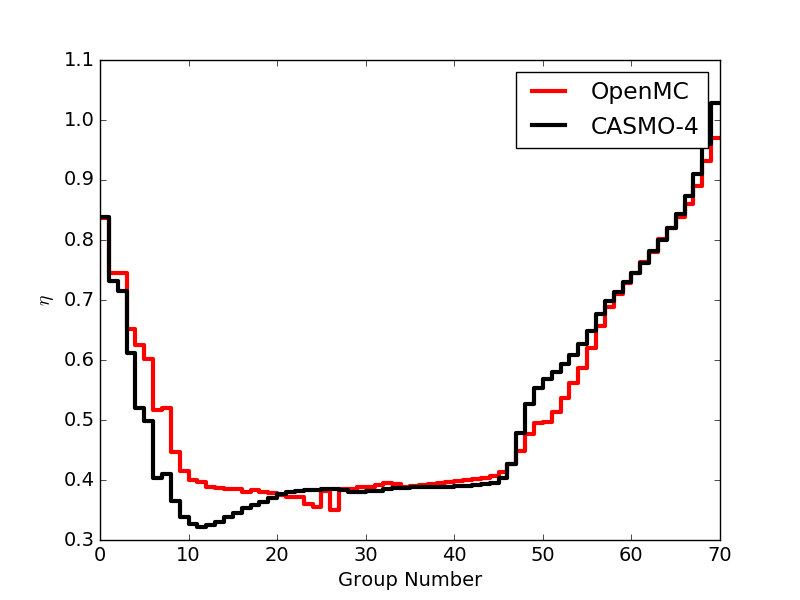
\includegraphics[width=0.7\linewidth]{figures/beavrs-visual/eta.png}
	\caption{A comparison of the $\eta$ factor defined in Eq.~\ref{eq:eta} for cross-sections generated with OpenMC and the CASMO-4 cross-sections for water in 70 energy groups.}
	\label{fig:eta}
\end{figure} 

In this appendix, the mechanics and theory behind multi-group cross-section generation were discussed. The focus was placed on Monte Carlo generation of cross-sections for full core simulation. In this process, it is important to highlight that while continuous energy cross-sections only depend on material properties, multi-group cross-sections are region-dependent due to dependence on the flux spectrum within each region. This effect can be quite significant. However, at large number of energy groups, the cross-sections more closely resemble the continuous energy cross-sections and the spatial dependence is diminished. This thesis concentrates on using a relatively large number of energy groups so that cross-sections can be treated as largely material dependent rather than having additional spatial dependence.



\end{appendices}
